\documentclass[a4paper, 12pt]{book}
\title{Machine Learning Specialization}
\author{Mohammad Parsa Bashari}
\date{January 2023}
\setlength{\parskip}{4pt}
\usepackage[margin=20mm]{geometry}
\usepackage{titlesec}
\usepackage{pgfplots}
\pgfplotsset{compat = newest}
\usepackage{amsmath}
\usepackage{algorithm}
\usepackage[noend]{algpseudocode}
\usepackage{listings}
\usepackage{graphicx}
\usepackage{amssymb}
% \usepackage{txfonts} % for italic small lambda
\usepackage{xcolor}
\definecolor{codegreen}{rgb}{0,0.6,0}
\definecolor{codegray}{rgb}{0.5,0.5,0.5}
\definecolor{codepurple}{rgb}{0.58,0,0.82}
\definecolor{backcolour}{rgb}{0.95,0.95,0.92}
\lstdefinestyle{mystyle}{
    backgroundcolor=\color{backcolour},   
    commentstyle=\color{codegreen},
    keywordstyle=\color{magenta},
    numberstyle=\tiny\color{codegray},
    stringstyle=\color{codepurple},
    basicstyle=\ttfamily\footnotesize,
    breakatwhitespace=false,         
    breaklines=true,                 
    captionpos=b,                    
    keepspaces=true,                 
    numbers=left,                    
    numbersep=5pt,                  
    showspaces=false,                
    showstringspaces=false,
    showtabs=false,                  
    tabsize=2
}
\usepackage{amssymb}% http://ctan.org/pkg/amssymb
\usepackage{pifont}% http://ctan.org/pkg/pifont
\newcommand{\cmark}{\ding{51}}
\newcommand{\xmark}{\ding{55}}
\lstset{style=mystyle}

\begin{document}
\thispagestyle{empty}
%% temporary titles
% command to provide stretchy vertical space in proportion
\newcommand\nbvspace[1][3]{\vspace*{\stretch{#1}}}
% allow some slack to avoid under/overfull boxes
\newcommand\nbstretchyspace{\spaceskip0.5em plus 0.25em minus 0.25em}
% To improve spacing on title pages
\newcommand{\nbtitlestretch}{\spaceskip0.6em}
\begin{center}
\bfseries
\nbvspace[1]
\Huge
{\nbtitlestretch\huge
MACHINE LEARNING SPECIALIZATION}

\nbvspace[1]
\normalsize

NOTES TAKEN FROM COURSERA'S \\
MACHINE LEARNING SPECIALIZATION COURSE \\
\nbvspace[2]
\normalsize BY\\
\Large PARSA BASHARI\\[2em]
\footnotesize DeepLearning.AI \& Stanford online\\Taught by Andrew Ng

\nbvspace[3]


\includegraphics[width=6.5in]{graphics/cover.png}
\nbvspace[3]
\normalsize

SUMMER 2023\\
\nbvspace[1]
\end{center}

\tableofcontents
\chapter{Supervised Machine Learning}
 \section{Week 1: Introduction to Machine Learning}
\textbf{Outline:}
\begin{itemize}
    \item Define machine learning
    \item Define supervised learning
    \item Define unsupervised learning
    \item Write and run Python code in Jupyter Notebooks
    \item Define a regression model
    \item Implement and visualize a cost function
    \item Implement gradient descent
    \item Optimize a regression model using gradient descent
\end{itemize}
 \subsection{Supervised vs Unsupervised Learning}
\begin{enumerate}
    \item \textbf{Supervised Learning}: Inputs have labels
    \begin{enumerate}
        \item \textbf{Regression}: To find the output of an input within infinite choices
        \item \textbf{Classification}: To find the \emph{category} of an input
    \end{enumerate}
    \item \textbf{Unsupervised Learning}: Inputs are only given (The outputs are not specified)
    \begin{enumerate}
        \item \textbf{Clustering}: To find groups in unlabeled inputs
        \item \textbf{Anomaly Detection}: To find an input that is not normal
        \item \textbf{Dimensionality Reduction}: To reduce the size of data without losing much information
    \end{enumerate}
\end{enumerate}
\subsection{Terminology}
\begin{itemize}
    \item Training Set: Data used to train the model
    \item $x$: "input" variable (\textbf{feature})
    \item $y$: "output" variable (\textbf{target})
    \item $(x, y)$: A training example
    \item $m$: The number of training examples
    \item $(x^{(i)}, y^{(i)})$: $i^{th}$ training example
    \item $f$: The \emph{model} function
    \item $\hat{y}$ or \emph{prediction}: The output of $f$ (estimated value of $y$)
\end{itemize}
\subsection{Linear Regression}
We define our model function $f$ as follows:\[f_{w,b}(x) = wx + b\] where $w$ and $b$ are some constants. Most of the time, we simplify this notation to the following format:\[f(x) = wx + b\] This model is called \textbf{univariate linear regression} due to the fact that there is only one input variable $x$ in our model. The numbers $w$ and $b$ are called \textbf{parameters}.
\subsection{Cost Function}
In order to measure the accuracy of our linear regression model function, we define the \emph{cost function} that calculates the average error of our model function. A fundamental and common cost function is defined as follows: \[J(w,b) = \frac{1}{2m} \sum_{i=1}^{m} (\hat{y}^{(i)} - y^{(i)})^2\] where $\hat{y}^{(i)}$ is the predicted value of our model function corresponding to the input $x^{(i)}$. So the above formula can be written as follows: \[J(w,b) = \frac{1}{2m} \sum_{i=1}^{m} (f_{w,b}(x^{(i)}) - y^{(i)})^2\] Note that our goal is to find some $w$ and $b$ to minimize the cost function $J(w,b)$.

As an example, assume that we are given a training set like this: \[\{(x,y)\} = \{(0,0),(1,1),(2,2),(3,3)\}\] that can be plotted as follows:
\begin{center}
    \begin{tikzpicture} []
    \begin{axis}[xlabel = {$x$}, ylabel = {$y$}]
        \addplot [domain = 0:3, samples = 4, only marks, mark=x, red, mark size=4pt] {x};
    \end{axis}
\end{tikzpicture}
\end{center}
It is obvious that the best approximation of this plot is the line $y = x$ that occurs when we chose $w = 1$ and $b = 0$. So we expect that the cost function is minimum in the point $(w,b) = (1,0)$. Now let's form the cost function as follows: \[J(w,b) = \frac{1}{8} \sum_{i=1}^{4} ((w-1)x^{(i)} + b)^2 = \frac{1}{4} (2 b^2 + 6 b (w - 1) + 7 (w - 1)^2)\] Then we can plot this cost function:
\begin{center}
    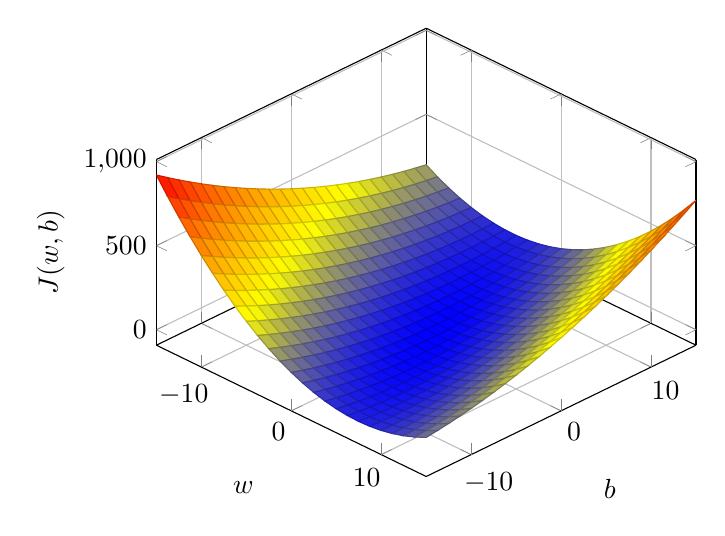
\begin{tikzpicture} []
    \begin{axis}[xlabel = {$w$},
        ylabel = {$b$},
        zlabel = {$J(w,b)$},
        view = {45}{45},
        grid]
        \addplot3 [
            domain = -15:15,
            domain y = -15:15,
            samples = 25,
            samples y = 25,
            surf] {(2*(y^2) + 6*y*(-1 + x) + 7*((-1 + x)^2))/4};
    \end{axis} 
\end{tikzpicture}
\end{center}
Another way to visualize the cost function is using a \textbf{contour plot}. This is the contour plot representation of the cost function above:
\begin{center}
    \begin{tikzpicture} []
    \begin{axis}[xlabel = {$w$},
        ylabel = {$b$},
        zlabel = {$J(w,b)$},
        view={0}{90},
        grid]
        \addplot3 [
            domain = -15:15,
            domain y = -15:15,
            samples = 100,
            samples y = 100,
            thick,
            contour gnuplot={levels={1,1.5,2,3,4,5}, labels=false}]
            {(2*(y^2) + 6*y*(-1 + x) + 7*((-1 + x)^2))/4};
    \end{axis} 
\end{tikzpicture}
\end{center}
\subsection{Gradient Descent}
Gradient Descent is an algorithm that is used to find a \emph{local minimum} of a function. The idea of gradient descent is to start from a point and each time, take a small step in the direction that lowers the cost more than other directions. The pseudocode of this algorithm is as follows:

\begin{algorithm}
\caption{Gradient Descent Algorithm}
\begin{algorithmic} [1]
\Repeat
\State $tmp\_w \gets w - \alpha{\frac{\partial}{\partial w}}f(w,b)$
\State $tmp\_b \gets b - \alpha{\frac{\partial}{\partial b}}f(w,b)$
\State $w \gets tmp\_w$
\State $b \gets tmp\_b$
\Until{convergence}
\end{algorithmic}
\end{algorithm}

The main part of this algorithm is to calculate the new $w$ and $b$. Note that $\alpha$ is called the \textbf{learning rate} which is an infinitesimal positive number that specifies the length of each step: \[w = w - \alpha {\frac{\partial}{\partial w}}f(w,b)\] \[b = b - \alpha {\frac{\partial}{\partial b}}f(w,b)\]

Note that if $\alpha$ is too small, the algorithm will work properly but it will be slow. If $\alpha$ is too large, gradient descent may fail to converge and never reach the minimum. Highlight the fact that as we approach the local minimum, gradient descent will take smaller steps because ${\frac{\partial}{\partial w}}f(w,b)$ and ${\frac{\partial}{\partial w}}f(w,b)$ get smaller.

Now let's use the gradient descent algorithm to find the proper $w$ and $b$ in the linear regression model. Recall that the model function is $f_{w,b}(x) = wx + b$, so we can calculate the partial derivatives with respect to $w$ and $b$: \[ \begin{split} {\frac{\partial}{\partial w}}J(w,b) & = \frac{\partial}{\partial w} (\frac{1}{2m} \sum_{i=1}^{m} (w{x^{(i)}} + b - y^{(i)})^2) \\ & = \frac{1}{m} \sum_{i=1}^{m} (w{x^{(i)}} + b - y^{(i)}){x^{(i)}}\end{split}\]
\[ \begin{split} {\frac{\partial}{\partial b}}J(w,b) & = \frac{\partial}{\partial b} (\frac{1}{2m} \sum_{i=1}^{m} (w{x^{(i)}} + b - y^{(i)})^2) \\ & = \frac{1}{m} \sum_{i=1}^{m} (w{x^{(i)}} + b - y^{(i)})\end{split}\]

In the linear regression model, the cost function always forms a \textbf{convex surface}\footnote{A surface that has a supporting plane (a plane that contains a point of the surface, but does not separate any two points of it) for each point on it.} that has only one local minimum which is also its global minimum. Thus, the gradient descent algorithm will always work if the learning rate is selected properly and also the initial value of $w$ and $b$ does not matter.

We call this procedure \textbf{Batch Gradient Descent} because each step of the algorithm uses all the training examples.
\section{Week 2: Regression with multiple variables}
This week, you'll extend linear regression to handle multiple input features. You'll also learn some methods for improving your model's training and performance, such as vectorization, feature scaling, feature engineering, and polynomial regression. At the end of the week, you'll get to practice implementing linear regression in code.
\subsection{Multiple Linear Regression}
Suppose that we want to implement a model that predicts the price of a house according to its size, its number of bedrooms, its number of floors, and its age. Obviously, here we have a model function with several inputs (features) and we have some new terminology:
\begin{itemize}
    \item $x_j$ : $j^{th}$ feature
    \item $n$ : The number of features
    \item $\Vec{x}^{(i)}$ : features of $i^{th}$ training example
    \item ${x_j}^{(i)}$ : value of the feature $j$ in $i^{th}$ training example
\end{itemize}
And our linear regression model function will look like this: \[f_{\Vec{w},b} (\Vec{x}) = w_1x_1 + w_2x_2 + ... + w_nx_n + b\] where $\Vec{w}$ and $b$ are the parameters of the model and $\Vec{x}$ is the input. Now we can rewrite the function $f$ using dot product: \[f_{\Vec{w},b} (\Vec{x}) = \Vec{w}.\Vec{x} + b\]
\subsection{Vectorization}
Vectorization is a way to do vector calculation faster in coding. The \lstinline{numpy} library supports vectorization and using its methods, we have to do vector calculation much faster than the naive implementation (e.g. using a \lstinline{for} loop). Now, look at the following two different implementations of $f_{\Vec{w},b} (\Vec{x})$ in python:

\begin{table}[h]
\noindent\begin{minipage}{.45\textwidth}
\begin{lstlisting}[language=Python, caption={without vectorization}]
def f(w, x, b):
    f = 0
    for i in range(n):
        f += w[i]*x[i]
    return f + b
\end{lstlisting}
\end{minipage}\hfill
\noindent\begin{minipage}{.45\textwidth}
\begin{lstlisting}[language=Python, caption={with vectorization}]
import numpy as np

def f(w, x, b):
    f = np.dot(w,x) + b
    return f
\end{lstlisting}
\end{minipage}
\end{table}

The reason for faster calculation in the vectorized environment is the use of parallel processing hardware. Now we can implement the gradient descent algorithm for multiple linear regression. Notice that the cost function is now in the form $J(\Vec{w},b)$ and returns a scalar. We have to calculate ${\frac{\partial}{\partial w_j}}f(\Vec{w},b)$ for $j$ from 1 to $n$. So each algorithm step will look like this: \[w_j = w_j - \alpha\frac{1}{m} \sum_{i=1}^{m} (\Vec{w}.\Vec{x}^{(i)} + b - y^{(i)})x_j^{(i)} \qquad\qquad j=1,2,...,n\] and b is updated just like in univariate linear regression.

\subsection{Feature Scaling}
Consider the situation where the features have different ranges. For instance, consider: \[300 feet^2 \leq x_1 \leq 2000 feet^2 , \qquad \qquad 0 \leq x_2 \leq 5\] where $x_1$ is the size of the house and $x_2$ is the number of bedrooms. In this case, when we run the gradient descent, the algorithm may jump multiple times before reaching the minimum point, because in the counter plot, the ovals are long and narrow.

To fix this issue, we scale the features such that their ranges become the same. For example, we can divide each feature by the maximum of its range. Thus in our example, we can scale as follows: \[x_{1, scaled} = \frac{x_1}{max_1} = \frac{x_1}{2000}, \qquad \qquad x_{2, scaled} = \frac{x_2}{max_2} = \frac{x_2}{5}\]

Another way to scale the features is called \textbf{Mean Normalization}. In this method, we scale features to the interval $\left[-1,1\right]$. To do this, we first find the average of each feature (say $\mu_1$, $\mu_2$, ...). Then we use the following relation to scale the features: \[x_{j, scaled} = \frac{x_j - \mu_j}{max_j - min_j}\]

The last method of feature scaling is called \textbf{Z-score Normalization}. In this method, in addition to the average, we calculate the \emph{standard deviation}, $\sigma$, and then we scale the feature as follows: \[x_{j, scaled} = \frac{x_j - \mu_j}{\sigma_j}\]

\subsection{Convergence Check for Gradient Descent}
We define the \textbf{Learning Curve} as a graph of the cost $J$ as a function of the number of iterations in the gradient descent algorithm. To check the convergence of the algorithm, we should check if the diagram is always decreasing. If the function is increasing at some point, it means that the learning rate $\alpha$ has been chosen improperly (i.e. too large).

Another way to check the convergence is called \textbf{Automatic Convergence Test}. Let $\epsilon$ be an infinitesimal number (say $10^{-3}$); Now if $J(\Vec{w},b)$ decreases by $\le \epsilon$ in one iteration, we find realize that the algorithm has converged. Due to the difficulties in choosing $\epsilon$, we use the learning curve much more than the automatic convergence check.

\subsection{Choosing the Learning Rate}
\begin{algorithm}
\caption{Choosing the Proper Learning Rate}
\begin{algorithmic} [1]
\State Let $\alpha$ be a very small value and test the algorithm
\If{diverges}
    \State there is a bug in the code
\Else
    \Repeat
    \State $\alpha \gets \approx 3\alpha$
    \Until{the algorithm converges \textbf{and} the decreasing rate is maximum}
\EndIf
\end{algorithmic}
\end{algorithm}

\subsection{Polynomial Regression}
What if your features/data are non-linear or are combinations of features? For example,  Housing prices do not tend to be linear with the living area but penalize very small or very large houses. How can we use the machinery of linear regression to fit this curve? Recall, the \emph{machinery} we have is the ability to modify the parameters $w$ and $b$ to \emph{fit} the equation to the training data. However, no amount of adjusting of $w$ and $b$ will achieve a fit to a non-linear curve.

In this situation, we create new features that are made of the main features. For instance, consider we have two base features $x_1$ and $x_2$. Then we can come up with a new feature $x_3$ where $x_3 = x_1x_2$. This process is called \textbf{Feature Engineering}. As a special case of feature engineering, if we choose the new feature as a power of a main feature, our model function will look like this: \[f_{\Vec{w},b}(x) = w_1x + w_2x^2 + w_3x^3 + ... + w_kx^k + b\] And this model is called \textbf{Polynomial Regression}.

\section{Week 3: Classification}
This week, you will learn the other type of supervised learning, classification. You will learn how to predict categories using the logistic regression model. You will learn about the problem of overfitting, and how to handle this problem with a method called regularization.

\subsection{Logistic Regression}
As we mentioned before, in the classification we want to choose between a limited number of choices. Each choice is called a \textbf{class} or a \textbf{category}. If the number of choices is two, then we call this problem, \textbf{Binary Classification}. In binary classification, we have two categories: \emph{negative class} and \emph{positive class}, in which the output $y$ is relatively 0 and 1.

It turns out that the linear regression model will not work properly for classification problems. So we introduce another model, called \textbf{Logistic Regression}. In order to implement logistic regression, we should be familiar with an important mathematical function called \textbf{Sigmoid Function} or \textbf{Logistic Function}, which is defined as follows\footnote{In the course, the Sigmoid/Logistic function is denoted as $g(x)$.}: \[S(x) = \frac{1}{1+e^{-x}}\] and is plotted like this:
\begin{center}
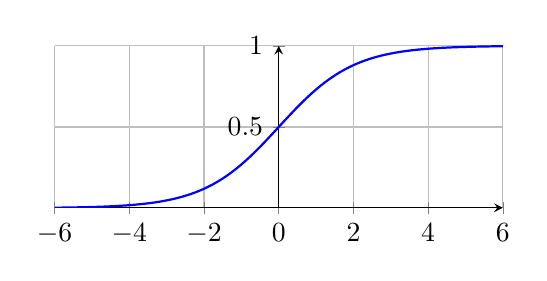
\begin{tikzpicture}
\begin{axis}
[
    grid=major,     
    xmin=-6,
    xmax=6,
    axis x line=bottom,
    ytick={0,.5,1},
    ymax=1,
    axis y line=middle,
    height=0.3\textwidth,
    width=0.6\textwidth
]
    \addplot
    [
        blue,
        mark=none,
        samples=100,
        domain=-6:6,
        thick
    ]
    (x,{1/(1+exp(-x))});
\end{axis}
\end{tikzpicture}
\end{center}

Now we can define the logistic regression model as follows: \[f_{\Vec{w},b}(\Vec{x}) = S(\Vec{w}.\Vec{x}+b) = \frac{1}{1+e^{-(\Vec{w}.\Vec{x}+b)}}\] where $S$ is the Sigmoid function. This function can be interpreted as the chance that $y$ is equal to 1. Therefore, the logistic regression model function is also written as \[f_{\Vec{w},b}(\Vec{x}) = P(y=1 | \Vec{x}; \Vec{w}, b)\] which is the probability that $y = 1$, given input $\Vec{x}$ and parameters $\Vec{w},b$.
\subsection{Decision Boundary}
The logistic regression model has to predict that y is equal to zero or one. Thus we need a threshold for the output of $f_{\Vec{w},b}(\Vec{x})$. By looking at the graph of the Sigmoid function, we find out that the output is greater than 0.5 if the input is greater than zero and the output is less than 0.5 if the input is less than zero. Therefore, if we choose 0.5 as the threshold of output, then we should compare $\Vec{w}.\Vec{x} + b$ with zero to predict the output of the model function. We define the line \[z = \Vec{w}.\Vec{x} + b = 0\] which is called the \textbf{Decision Boundary}. Consider the case that we have two features ($x_1$ and $x_2$) and a dataset like this:
\begin{center}
    \begin{tikzpicture} [scale=0.8]
    \begin{axis}[
        xlabel = {$x_1$},
        ylabel = {$x_2$},
        scatter/classes={
        a={mark=o,draw=blue, mark size=3pt},
        b={mark=x,draw=red, mark size=4pt}}]
        \addplot+[scatter, only marks, scatter src=explicit symbolic] table[meta=label] {data/1.3.2.dat};
    \end{axis}
\end{tikzpicture}
\end{center}
Then the decision boundary is the line below when $w_1 = 1$, $w_2 = 1$, and $b = -3$: \[z = w_1x_1 + w_2x_2 + b = 0 \implies x_1 + x_2 = 3\]
which is the purple line in the following diagram:
\begin{center}
    \begin{tikzpicture} [scale=0.8]
    \begin{axis}[
        grid=major,
        grid style=dashed,
        xlabel = {$x_1$},
        ylabel = {$x_2$},
        scatter/classes={
        a={mark=o,draw=blue, mark size=3pt},
        b={mark=x,draw=red, mark size=4pt}}]
        \addplot+[scatter, only marks, scatter src=explicit symbolic] table[meta=label] {data/1.3.2.dat};
        \addplot[samples=40, purple, domain=-0.3:3.3, thick] {3 - x};
    \end{axis}
\end{tikzpicture}
\end{center}
Recall from section 1.2.6, we can employ feature engineering (and especially polynomial regression) to form complex nonlinear decision boundary curves using additional features.
\subsection{Cost Function for Logistic Regression}
It turns out that if we chose the squared error cost function for logistic regression, the generated curve is not a vertex curve, thus it has more than one local minimum and the gradient descent will fail. Now we introduce another cost function to solve this issue. First, let's define the \textbf{Loss Function} as follows:
\[L(f_{\Vec{w},b}(\Vec{x}^{(i)}), y^{(i)}) = 
\begin{cases}
    -\log(f_{\Vec{w},b}(\Vec{x}^{(i)})) &\quad y^{(i)} = 1 \\
    -\log(1 - f_{\Vec{w},b}(\Vec{x}^{(i)})) &\quad y^{(i)} = 0
\end{cases}
\]
This function describes how the model function predicts \emph{a single training example}. Let's plot the loss function. Note that the domain is $(0,1)$ because the Sigmoid function only creates values between 0 and 1:
\begin{center}
    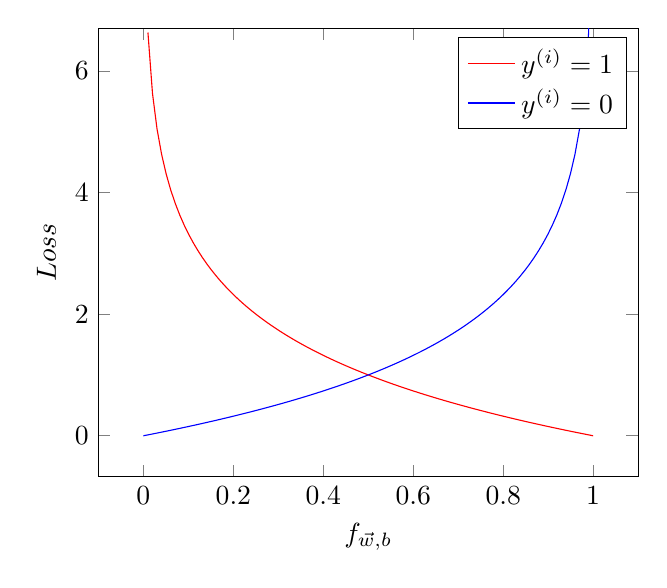
\begin{tikzpicture} []
    \begin{axis}[xlabel = {$f_{\Vec{w},b}$},
                ylabel = {$Loss$},
                ymax=6.7]
        \addplot [domain = 0:1, samples = 100, red] {-log2(x)};
        \addlegendentry{\(y^{(i)} = 1\)}
        \addplot [domain = 0:1, samples = 100, blue] {-log2(1 - x)};
        \addlegendentry{\(y^{(i)} = 0\)}
    \end{axis}
\end{tikzpicture}
\end{center}
You can check in both cases that the further the prediction $f_{\Vec{w},b}(\Vec{x}^{(i)})$ is from target $y^{(i)}$, the higher the loss. Now we can define the new cost function for logistic regression as follows: \[J(\Vec{w},b) = \frac{1}{m}\sum_{i=1}^{m} L(f_{\Vec{w},b}(\Vec{x}^{(i)}), y^{(i)})\] which turns out that will generate a convex curve on which the gradient descent will work properly. According to the fact that $y^{(i)}$ can only be 0 or 1, we can simplify the loss function above and write it as follows: \[L(f_{\Vec{w},b}(\Vec{x}^{(i)}), y^{(i)}) = -y^{(i)}\log(f_{\Vec{w},b}(\Vec{x}^{(i)})) - (1-y^{(i)})\log(1 - f_{\Vec{w},b}(\Vec{x}^{(i)}))\] which is much easier in implementation. Eventually, the cost function for logistic regression is calculated as follows: \[J(\Vec{w},b) = -\frac{1}{m}\sum_{i=1}^{m} y^{(i)}\log(f_{\Vec{w},b}(\Vec{x}^{(i)})) + (1-y^{(i)})\log(1 - f_{\Vec{w},b}(\Vec{x}^{(i)}))\] which is widely used today for logistic regression cost calculation.
\newpage
\subsection{Gradient Descent for Logistic Regression}
Although the cost function for logistic regression is different from the one used for linear regression, if we differentiate from the cost function with respect to $w_j$ and $b$ (for $j=1,...,n$), the result is the same as in the linear regression case:
\[{\frac{\partial}{\partial w_j}}J(\Vec{w},b) = \frac{1}{m} \sum_{i=1}^{m} (f_{\Vec{w},b}(\Vec{x}^{(i)}) - y^{(i)})x_j^{(i)}\]
\[{\frac{\partial}{\partial b}}J(\Vec{w},b) = \frac{1}{m} \sum_{i=1}^{m} (f_{\Vec{w},b}(\Vec{x}^{(i)}) - y^{(i)})\]
which are absolutely the same equations as the equations in section 1.1.5, but with a different model function $f_{\Vec{w},b}(\Vec{x}^{(i)})$.
\subsection{The Problem of Overfitting}
As mentioned in section 1.2.6, by feature engineering we can add new features that are made by combining the previous features to help our model function to fit the training set better. It turns out that if we overdo feature engineering, it will cause a problem called \textbf{overfitting} or \textbf{high variance} in our model. For instance, if we choose a $6^{th}$ order polynomial function for a training set that can be modeled by a $2^{nd}$ order polynomial, then we come up with a wiggly curve that fits the training data very well but does not work well with new inputs. The \emph{high variance} term has come from the fact that in the overfit case if we change only a single training example, we come up with a completely different function that predicts a completely different output for the same new input.

On the other hand, if we take our model function too simple, it does not fit the training set very well and also does not work properly with new inputs. We call this situation \textbf{underfitting} or \textbf{high bias}. Our goal is to find a model function that does neither overfit nor underfit the training set which we call \textbf{generalized} model. In the following table, you can see the summary of this section.
\renewcommand{\arraystretch}{1.8}
\begin{center}
\begin{tabular}{|c||c|c|c|}
    \hline
    Case & Simplicity & Fitting Training Set & Predicting New Examples \\
    \hline \hline
    underfit/high bias & \cmark & \xmark & \xmark \\
    \hline
    generalized & \textbf{-} & \textbf{-} & \cmark \\
    \hline
    overfit/high variance & \xmark & \cmark & \textbf{-} \\
    \hline
\end{tabular}
\end{center}

\subsubsection{Addressing Overfitting}
To address the overfitting problem, the following steps may help:
\begin{enumerate}
    \item Add more training examples
    \item Only select useful features when insufficient training examples are available (Feature Selection)
    \item Reduce the size of parameters by \emph{regularization}
\end{enumerate}

\subsection{Regularization}
Regularization is a technique to reduce the problem of overfitting. The main idea of regularization is that we decrease the parameters $w_j$ to lower the effect of each feature on the ultimate function. To achieve this, we add a penalty to the cost function to penalize the model if the parameters are getting big. Here is our new regularized cost function in both linear and logistic regression: \[J_{reg}(w,b) = J(w,b) + \frac{\lambda}{2m} \sum_{j=1}^{n} w_j^2\] where $\lambda$ is called the \textbf{regularization parameter}. Note that regularizing the parameter $b$ is optional and is often omitted.

\chapter{Advanced Learning Algorithms}
\section{Week 1: Neural Networks}
This week, you'll learn about neural networks and how to use them for classification tasks. You'll use the TensorFlow framework to build a neural network with just a few lines of code. Then, dive deeper by learning how to code up your own neural network in Python, "from scratch". Optionally, you can learn more about how neural network computations are implemented efficiently using parallel processing (vectorization).
\subsection{Neural Networks Intuition}
To mimic the functionality of the human brain, we model each neuron as a node that gets some inputs and gives an output called \textbf{activation} which is sent to the next node (neuron). As an example, assume that we want to predict if a T-shirt will be a top seller. Then we design a neural network like this:
\begin{center}
    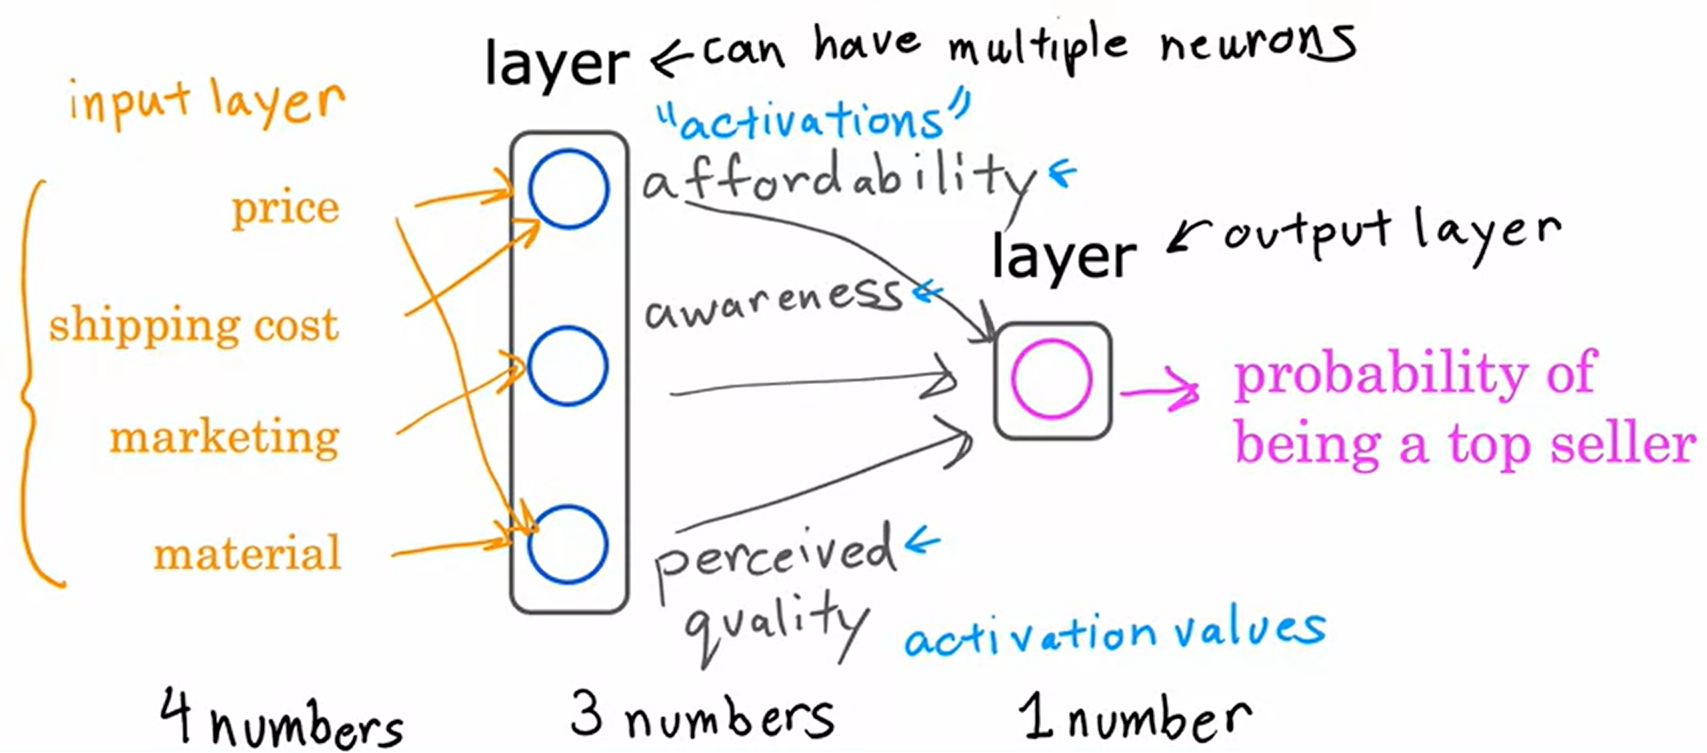
\includegraphics[width=6in]{graphics/NN-Intuition.png}
\end{center}
we call the middle layer the \textbf{hidden layer}. We can show the input layer as a vector $\Vec{x}$, the hidden layer as $\Vec{a}$, and the output layer as a scalar $a$. Note that in a neural network system, the hidden layers are designed by the algorithm itself and we are not responsible to do anything about that.
\subsection{Neural Network Model}
Neural network models can have multiple hidden layers. The layer associated with a particular variable is denoted by the superscript $[l]$. For instance, the activation value of layer $l$ and unit(neuron) $j$ is calculated as follows: \[\Vec{a}_j^{[l]} = S(\Vec{w}_j^{[l]}.\Vec{a}_j^{[l-1]} + b_j^{[l]}) = \frac{1}{1 - e^{-(j^{[l]}.\Vec{a}_j^{[l-1]} + b_j^{[l]})}}\] where $S$ is the Sigmoid or logistic function which is called the \textbf{activation function} because it creates the activation value of a layer. Note that according to this notation, the input layer is denoted as $a^{[0]}$ to make the relation above work correctly for any value of $l$. A famous neural network architecture where each layer has fewer units than the previous one is called \textbf{forward propagation}.

\subsection{Implementing Forward Propagation}
Here is the implementation of a single layer neural network in two different ways:
\begin{lstlisting}[language=Python, caption={without vectorization}]
import numpy as np

def my_dense(a_in, W, b, g):
    """
    Args:
      a_in (ndarray (n, )) : Data, 1 example 
      W    (ndarray (n,j)) : Weight matrix, n features per unit, j units
      b    (ndarray (j, )) : bias vector, j units  
      g    activation function (e.g. sigmoid, relu..)
    Returns
      a_out (ndarray (j,))  : j units
    """
    units = W.shape[1]
    a_out = np.zeros(units)
    for j in range(units):
        z = np.dot(W[:, j], a_in) + b[j]
        a_out[j] = g(z)   
    return(a_out)
\end{lstlisting}

\begin{lstlisting}[language=Python, caption={with vectorization}]
import numpy as np

def my_dense_v(A_in, W, b, g):
    """
    Computes dense layer
    Args:
      A_in (ndarray (m,n)) : Data, m examples, n features each
      W    (ndarray (n,j)) : Weight matrix, n features per unit, j units
      b    (ndarray (1,j)) : bias vector, j units  
      g    activation function (e.g. sigmoid, relu..)
    Returns
      A_out (tf.Tensor or ndarray (m,j)) : m examples, j units
    """
    Z = np.matmul(A_in, W) + b
    A_out = g(Z)
    return(A_out)
\end{lstlisting}

\section{Week 2: Neural Network Training}
This week, you'll learn how to train your model in TensorFlow, and also learn about other important activation functions (besides the sigmoid function), and where to use each type in a neural network. You'll also learn how to go beyond binary classification to multiclass classification (3 or more categories). Multiclass classification will introduce you to a new activation function and a new loss function. Optionally, you can also learn about the difference between multiclass classification and multi-label classification. You'll learn about the Adam optimizer, and why it's an improvement upon regular gradient descent for neural network training. Finally, you will get a brief introduction to other layer types besides the one you've seen thus far.

\subsection{Implementation in TensorFlow}
Here are the steps to implement a neural network model in TensorFlow:
\begin{lstlisting}[language=Python, caption={TensorFlow implementation}]
# specify the model and its structure
model = Sequential([
    Dense(units=25, activation='sigmoid'),
    Dense(units=15, activation='sigmoid'),
    Dense(units=1, activation='sigmoid')
])

# determine the loss and cost function
model.compile(loss=BinaryCrossentropy())

# train the data by repeating the algorithm 100 times
model.fit(X, y, epochs=100)
\end{lstlisting}

\subsection{Other Activation Functions}
Some famous activation functions are the following:
\begin{table}[ht]
\noindent
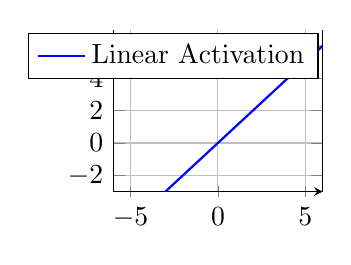
\begin{tikzpicture}
\begin{axis}
[
    grid=major,     
    xmin=-6,
    xmax=6,
    axis x line=bottom,
    ymax=7,
    ymin=-3,
    height=0.3\textwidth,
    width=0.35\textwidth
]
    \addplot
    [
        blue,
        mark=none,
        samples=100,
        domain=-6:6,
        thick
    ]
    (x,x);
    \addlegendentry{Linear Activation}
\end{axis}
\end{tikzpicture}
\hfill
\noindent
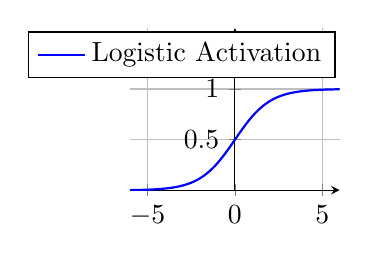
\begin{tikzpicture}
\begin{axis}
[
    grid=major,     
    xmin=-6,
    xmax=6,
    axis x line=bottom,
    ytick={0,.5,1},
    ymax=1.6,
    axis y line=middle,
    height=0.3\textwidth,
    width=0.35\textwidth
]
    \addplot
    [
        blue,
        mark=none,
        samples=100,
        domain=-6:6,
        thick
    ]
    (x,{1/(1+exp(-x))});
    \addlegendentry{Logistic Activation}
\end{axis}
\end{tikzpicture}
\hfill
\noindent
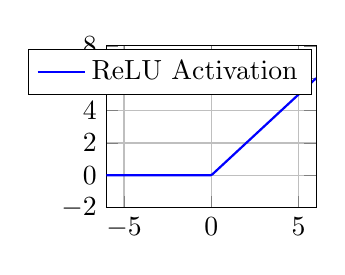
\begin{tikzpicture}
\begin{axis}
[
    grid=major,     
    xmin=-6,
    xmax=6,
    ymax=8,
    ymin=-2,
    height=0.3\textwidth,
    width=0.35\textwidth
]
    \addplot
    [
        blue,
        mark=none,
        samples=100,
        domain=-6:6,
        thick
    ]
    (x,{max(0,x)});
    \addlegendentry{ReLU Activation}
\end{axis}
\end{tikzpicture}
\end{table}

\noindent where the ReLU (Rectified Linear Unit) activation is defined as \[g(z) = max(0,z)\]
It is important to learn how to choose an activation function. We first decide about the output layer. Here is a guide:
\begin{center}
    \begin{tabular}{|c|c|c|}
        \hline
        Case & Range of Output & Preferred Activation Function\\
        \hline \hline
        Binary Classification & 0 or 1 & Logistic Activation \\
        \hline
        Regression & - or + & Linear Activation \\
        \hline
        Regression & 0 or + & ReLU Activation \\
        \hline
    \end{tabular}
\end{center}
For the hidden layers, it turns out that the ReLU activation function is the most common choice compared to the logistic function. Here are some benefits of the ReLU over the logistic activation function:
\begin{enumerate}
    \item It is faster to calculate.
    \item It is faster to learn (because of having less \textbf{flat} parts than the logistic function).
\end{enumerate}
Note that the linear activation function can not be used in hidden layers, Because this is completely equivalent to using normal linear or logistic regression.

\subsection{Multiclass Classification}
In multiclass classification, the output $y$ can get $N > 2$ discrete values. In order to do this, we use an algorithm called \textbf{Softmax Regression}. Suppose that the output $y$ can get the values $\{1,2,3,...,N\}$ and let $a_j$ be the probability that $y$ equals $j$ (for $j = 1,2,...,N$). The parameters of this model are $\Vec{w_j}$ and $b_j$ (for $j = 1,2,...,N$). According to these definitions, the softmax regression algorithm works as follows:
\[z_j = \Vec{w_j}.\Vec{x} + b_j \qquad \qquad a_j = \frac{e^{z_j}}{\sum_{i=1}^{N} e^{z_i}}\]
Note that the probabilities must sum up to one. So, \[a_1 + a_2 + ... + a_N = 1\]
The loss function here is derived from the case $N = 2$ (logistic regression):
\[ L(a_1,a_2,...,a_N,y) =
\begin{cases}
    -\log a_1 &\quad y = 1 \\
    -\log a_2 &\quad y = 2 \\
    \qquad \vdots & \\
    -\log a_N &\quad y = N
\end{cases}
\]
\subsection{Neural Network with Softmax Output}
In order to implement a multiclass classification with a neural network, we can just let the output layer have $N$ units. In TensorFlow, we can implement it just by changing the last layer's activation and the loss function. But there is a better way to implement this. We can let the last layer's activation be \emph{linear} (i.e. return the $z_j$s, not $a_j$s). And then add something to the loss function to tell it about our decision. The code for both implementations is provided in the next page.

\begin{lstlisting}[language=Python, caption={normal implementation}]
model = Sequential(
    [ 
        Dense(25, activation = 'relu'),
        Dense(15, activation = 'relu'),
        Dense(4, activation = 'softmax')    # softmax activation here
    ]
)
model.compile(
    loss=tf.keras.losses.SparseCategoricalCrossentropy(),
    optimizer=tf.keras.optimizers.Adam(0.001),
)
model.fit(
    X_train,y_train,
    epochs=10
)
\end{lstlisting}
\begin{lstlisting}[language=Python, caption={preferred implementation}]
preferred_model = Sequential(
    [ 
        Dense(25, activation = 'relu'),
        Dense(15, activation = 'relu'),
        Dense(4, activation = 'linear')
    ]
)
preferred_model.compile(
    loss=tf.keras.losses.SparseCategoricalCrossentropy(from_logits=True),
    optimizer=tf.keras.optimizers.Adam(0.001),
)
preferred_model.fit(
    X_train,y_train,
    epochs=10
)
\end{lstlisting}

\subsection{Adam Algorithm and Convolutional Neural Network}
\subsubsection{Adam Algorithm}
You may have wondered about the additional argument passed into \emph{compile()} function. The \textbf{Adam Algorithm} \footnote{Adaptive Moment Estimation} is an optimization to the gradient descent algorithm. It makes the gradient descent faster by using different learning rates for different parameters of the model.

\subsubsection{Convolutional Neural Network}
In normal layers, each unit uses all elements of the input vector (activations of the previous layer). But it turns out that if each unit of a layer uses only a partition of the previous layer's output, it will yield some benefits. For instance:
\begin{itemize}
    \item the computations are faster
    \item the model needs less training data
    \item less prone to overfitting
\end{itemize}

\section{Week 3: Advice for Applying Machine Learning}
This week you'll learn best practices for training and evaluating your learning algorithms to improve performance. This will cover a wide range of helpful advice about the machine learning life-cycle, tuning your model, and also improving your training data.

\subsection{Model Evaluation}
A technique for evaluating a model is to divide the training data into two subsets; \textbf{training set} and \textbf{test set} (e.g. $70\%$ to $30\%$). Then by calculating \emph{test error} and \emph{training error} we are able to evaluate the functionality of our model. Suppose that $m_{train}$ and $m_{test}$ are respectively the size of the training set and the test set.

In linear regression, the cost function is defined as follows (recall from 1.3.6):
\[J(\Vec{w},b) = \left[\frac{1}{2m_{train}} \sum_{i=1}^{m_{train}} (f_{w,b}(\Vec{x}^{(i)}) - y^{(i)})^2 + \frac{\lambda}{2m_{train}} \sum_{j=1}^{n} w_j^2\right]\]
Then the test error is calculated as follows:
\[J_{test}(\Vec{w},b) = \frac{1}{2m_{test}} \left[ \sum_{i=1}^{m_{test}} (f_{w,b}(\Vec{x}_{test}^{(i)}) - y_{test}^{(i)})^2\right]\]
And the training error is:
\[J_{train}(\Vec{w}, b) = \frac{1}{2m_{train}} \left[ \sum_{i=1}^{m_{train}} (f_{w,b}(\Vec{x}_{train}^{(i)}) - y_{train}^{(i)})^2\right]\]
Now if we look at $J_{test}(\Vec{w},b)$ and $J_{train}(\Vec{w},b)$, we can come up with some consequences. If $J_{train}(\Vec{w},b)$ is high, then our model is underfitted. If $J_{train}(\Vec{w},b)$ is low ($\approx 0$) but $J_{test}(\Vec{w},b)$ is high, then our model is overfitted.

In classification problems, although we could use the above approach, there is a simpler and more common way to evaluate a classification model. In this approach, we define $J_{train}(\Vec{w},b)$ and $J_{test}(\Vec{w},b)$ as the fraction of the train/test set that has been misclassified. Then we can analyze our model in the same way as in linear regression.

After we chose the best model (the lowest $J_{test}$) if we want to report how well our selected model is performing, the test set is not a good indicator. In order to solve this issue, we change the process of training/testing a little bit by dividing our data into three parts (training set(60\%), \textbf{cross-validation set}(20\%), and test set(20\%)). The cross-validation set is also called \emph{validation set}, \emph{development set}, or \emph{dev set}. Then the cross-validation error is calculated as follows:
\[J_{cv}(\Vec{w}, b) = \frac{1}{2m_{cv}} \left[ \sum_{i=1}^{m_{cv}} (f_{w,b}(\Vec{x}_{cv}^{(i)}) - y_{cv}^{(i)})^2\right]\]
Then in order to choose a model, we look at $J_{cv}$ of our models and pick the lowest one. Then to report the estimate generalization error, we report $J_{test}$.
\newpage
\subsection{Bias and Variance}
If we try to plot $J_{cv}(\Vec{w},b)$ and $J_{train}(\Vec{w},b)$ with respect to the degree of the polynomial, we get something like this:
\begin{center}
    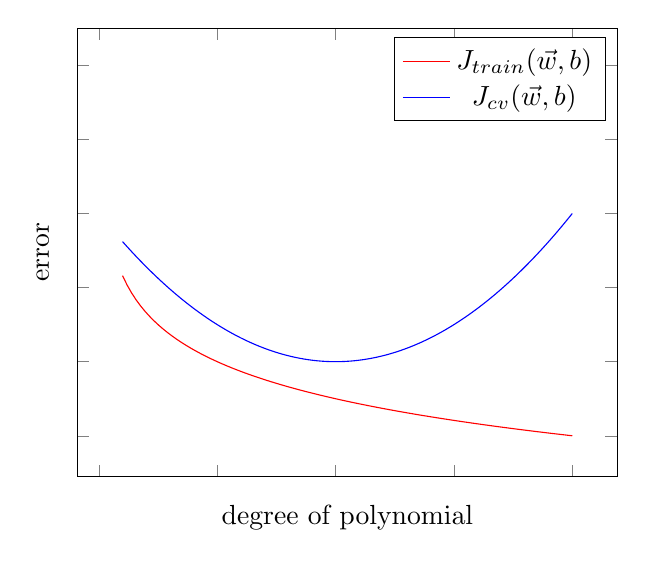
\begin{tikzpicture} []
    \begin{axis}[xlabel = {degree of polynomial},
                ylabel = {error},
                ymax=9,
                yticklabels={,,},
                xticklabels={,,}]
        \addplot [domain = 0.2:4, samples = 100, red] {-log2(x)};
        \addlegendentry{\(J_{train}(\Vec{w},b)\)}
        \addplot [domain = 0.2:4, samples = 100, blue] {(x-2)^2};
        \addlegendentry{\(J_{cv}(\Vec{w},b)\)}
    \end{axis}
\end{tikzpicture}
\end{center}
Now where $J_{train}$ is high ($J_{train} \approx J_{cv}$), we have \textbf{high bias} (underfit), and where $J_{train}$ is low and $J_{cv} \gg J_{train}$, we have \textbf{high variance} (overfit).

We can also use this approach to choose the best regularization parameter $\lambda$. If we plot $J_{cv}(\Vec{w},b)$ and $J_{train}(\Vec{w},b)$ with respect to $\lambda$, we get something like this:
\begin{center}
    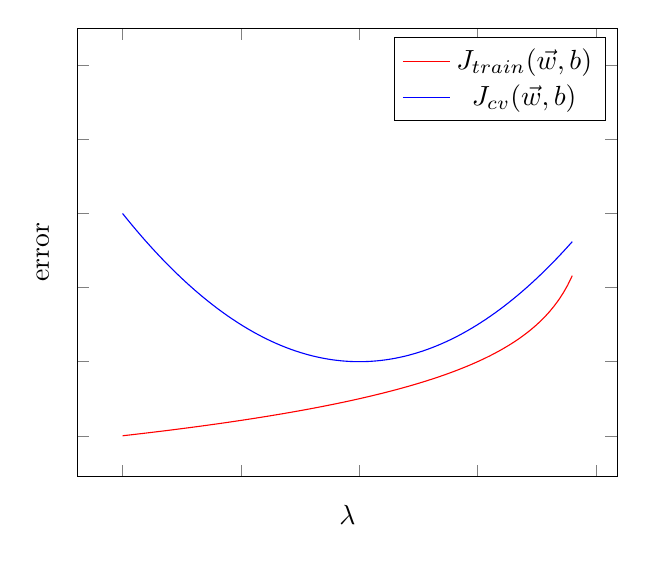
\begin{tikzpicture} []
    \begin{axis}[xlabel = {$\lambda$},
                ylabel = {error},
                ymax=9,
                yticklabels={,,},
                xticklabels={,,}]
        \addplot [domain = 0:3.8, samples = 100, red] {-log2(4-x)};
        \addlegendentry{\(J_{train}(\Vec{w},b)\)}
        \addplot [domain = 0:3.8, samples = 100, blue] {(x-2)^2};
        \addlegendentry{\(J_{cv}(\Vec{w},b)\)}
    \end{axis}
\end{tikzpicture}
\end{center}
And we can apply the previous conclusions in the case of choosing $\lambda$, too.

But when we talked about \emph{"high"} or \emph{"low"} error so far, what exactly did we mean? In order to specify a concrete definition of high and low, we should establish a baseline level of performance. There are some ways to do this:
\begin{itemize}
    \item Human-level performance
    \item Competing algorithms performance
    \item Guess based on experience
\end{itemize}
Then the two key quantities to measure are the difference between the training error and the baseline error, and the difference between the training error and the cross-validation error. According to these quantities, we can analyze our model the same as before.

\subsubsection{Learning Curve}
A learning curve is the functionality of our model in the case of different training set sizes. In general, if we plot the error of our model with respect to $m_{train}$, we get something like this:

\begin{center}
    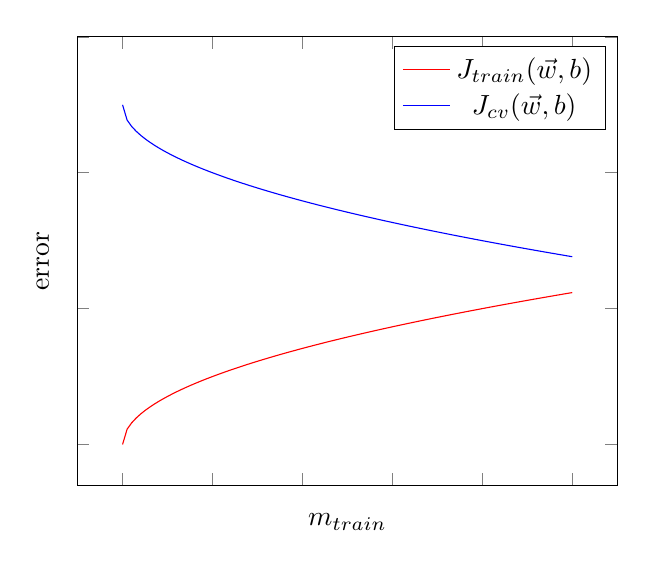
\begin{tikzpicture} []
    \begin{axis}[xlabel = {$m_{train}$},
                ylabel = {error},
                ymax=6,
                yticklabels={,,},
                xticklabels={,,}]
        \addplot [domain = 0:5, samples = 100, red] {sqrt(x)};
        \addlegendentry{\(J_{train}(\Vec{w},b)\)}
        \addplot [domain = 0:5, samples = 100, blue] {-sqrt(x) + 5};
        \addlegendentry{\(J_{cv}(\Vec{w},b)\)}
    \end{axis}
\end{tikzpicture}
\end{center}
\textbf{NOTE:} If a learning algorithm suffers from high bias, getting more training data will not (by itself) help much (the plot will be flattened out after a specific point). But in the high variance case, getting more training data is likely to help.

\subsection{Debugging a Learning Algorithm}
Here is a guide for what to do next. If your model has \textbf{high variance}, then:
\begin{itemize}
    \item Get more training examples
    \item Try smaller sets of feature
    \item Try increasing $\lambda$
\end{itemize}
and if your model has \textbf{high bias}, then:
\begin{itemize}
    \item Try getting additional features
    \item Try adding polynomial features
    \item Try decreasing $\lambda$
\end{itemize}

\subsubsection{Neural Networks and Bias/Variance}
\textbf{KEY NOTE}: Large neural networks are low-bias machines.

\noindent So there is a simple recipe that doesn't always work but is powerful when it does. The pseudo-code of this algorithm is given on the next page.
\newpage
\begin{algorithm}
\caption{Debugging High Bias and Variance in Neural Networks}
\begin{algorithmic} [1]
\State Train the model
\If{$J_{train}$ is high}
    \State Bigger network
    \State Go to line 1
\EndIf
\If{$J_{cv}$ is high}
    \State More data
    \State Go to line 1
\Else
    \State Done!
\EndIf
\end{algorithmic}
\end{algorithm}
A large neural network will usually do as well or better than a smaller one so long as regularization is chosen appropriately. In practice, to add regularization to a neural network layer, we can use the following piece of code:
\begin{lstlisting}[language=Python, caption={neural network regularization}]
layer = Dense(units=25, activation="relu", kernel_regularizer=L2(0.01))
\end{lstlisting}

\subsection{Machine Learning Development Process}
The development process of an ML project has an iterative loop like this:
\begin{center}
    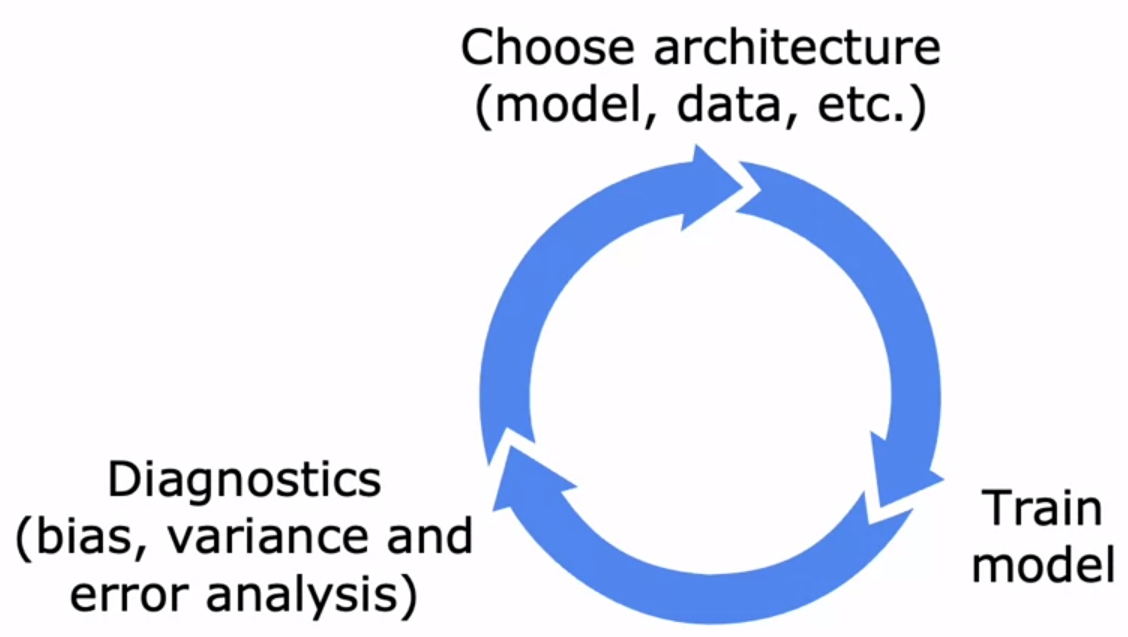
\includegraphics[width=3in]{graphics/ML_dev_loop.png}
\end{center}
In the error analysis step, we can manually examine the misclassified examples in the cross-validation set and categorize them based on common traits. This will help a lot in deciding what to do next. For example, you can collect more data with a specific property that had been seen a lot in the misclassified examples.

\textbf{Data Augmentation} is a data-collecting technique that modifies an existing training example to create a new training example. For instance, if we are developing a character recognition model and we have an image of the letter \emph{A}, then we can rotate, enlarge, shrink, or mirror the image and create new training examples with different input but the same output label. As another example, in a speech recognition model, we can add noisy background sounds to the input and make new examples with the same output sentence.

During the past decades, most machine learning researchers' attention was on the \textbf{conventional model-centric approach} which means the algorithm/model itself. Thanks to that paradigm of ML research, there are algorithms that are already very good and will work well for many applications. So, sometimes it can be more fruitful to spend more time taking a \textbf{data-centric approach} in which you focus on data collection and augmentation.

\subsection{Transfer Learning}
Imagine you want to build an ML system to recognize handwritten digits, but you don't have enough training examples. The idea of transfer learning is to take a model which has been trained before and use it in order to make your model work. For instance, assume that you have a million images (irrelevant to your model) like cats, dogs, cars, etc. which are from 1000 classes. The transfer learning process contains two steps:

\textbf{Supervised Pretraining:} In his step, you build a neural network (e.g. with 5 layers) with 1000 output units in the last layer. Then you train it with the million images you got from different objects. At the end of this step, you have parameters $W^{[1]},\Vec{b}^{[1]}$ to $W^{[5]},\Vec{b}^{[5]}$ where the dimension of the last layer parameters ($W^{[5]},\Vec{b}^{[5]}$) is 1000.

\textbf{Fine Tuning:} In this step, you copy the neural network from the previous step except for the output layer which has a different number of units (e.g. 10 for digit recognition) here. Then, If your training set is very small, you only train the output layer's parameters. But in the case that the training set is a bit bigger, you can train all parameters.

\subsection{Deployment}
The full cycle of a machine learning project is something like this:
\begin{center}
    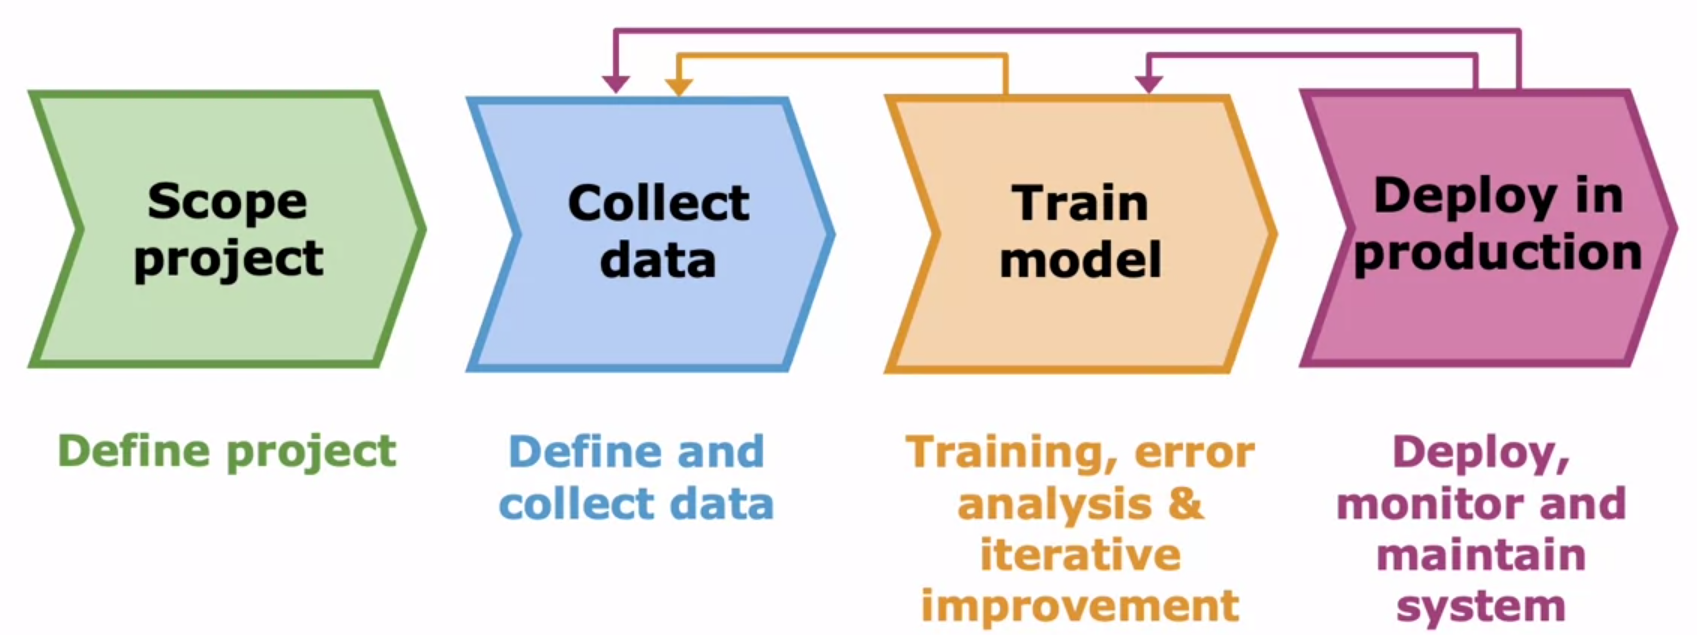
\includegraphics[width=4in]{graphics/Full_Cycle.png}
\end{center}
The most common way to deploy an ML system is to put it on a server and develop a client (a website or mobile app). When the client calls an API, the server passes the input to the ML system and gets the output (prediction $\hat{y}$). Then it sends the result to the client to be shown to the user. Note that this process requires software engineers to be developed, maintained, and monitor.

\subsection{Skewed Datasets}
A dataset is called \emph{skewed} if the number of positive examples is a lot more than the negative examples or vice versa. In this case, the error metrics are a bit different:

\begin{center}
    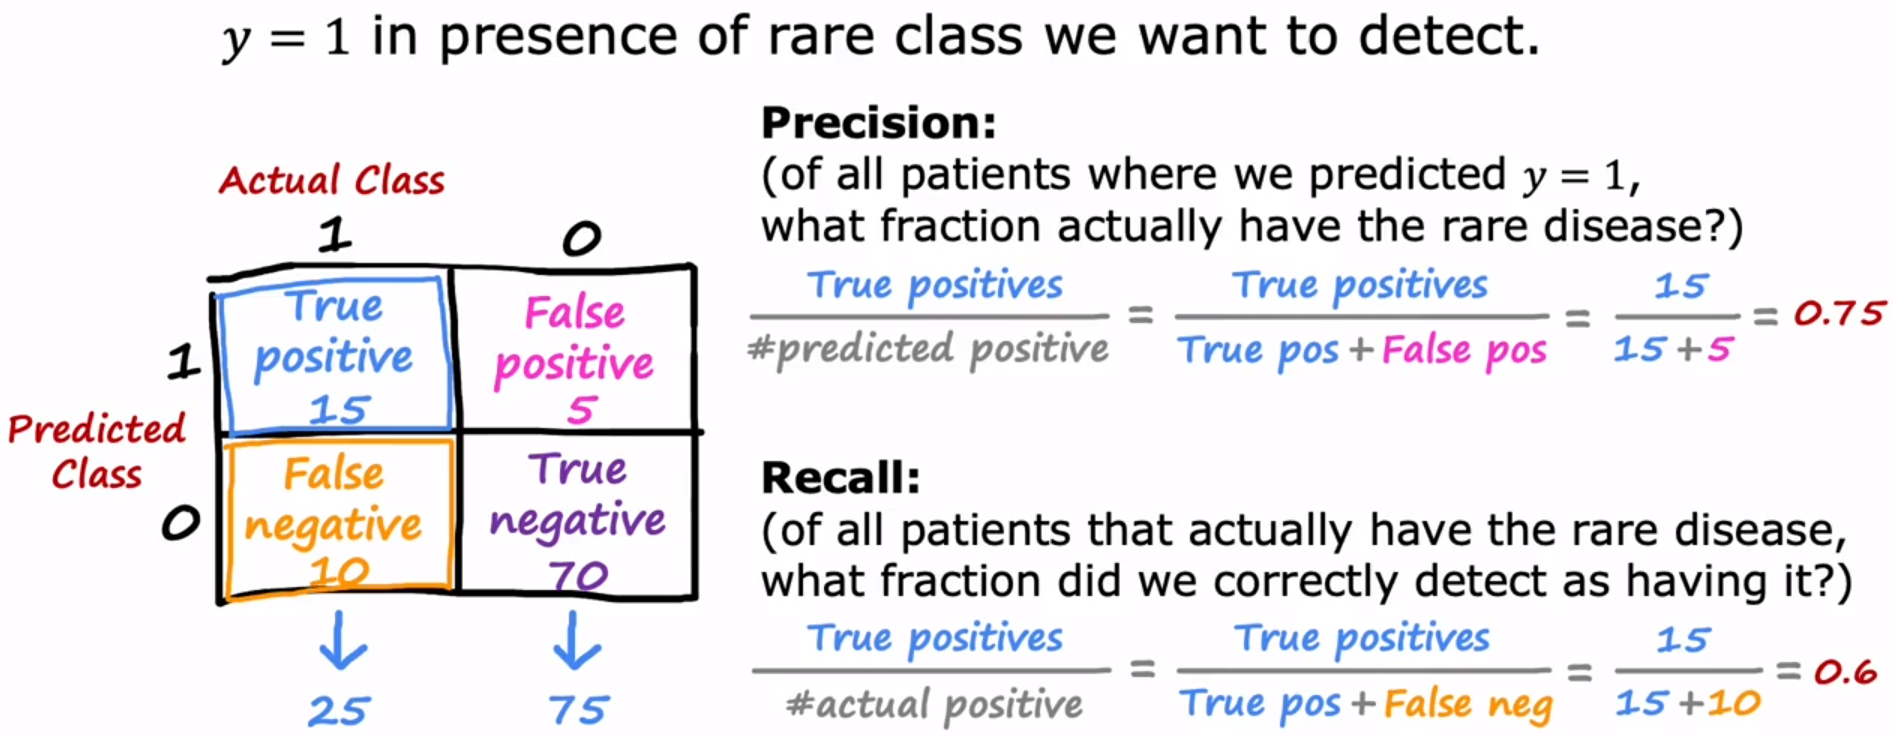
\includegraphics[width=5.5in]{graphics/skewed_dataset.png}
\end{center}
It turns out that there is a trade-off between precision and recall that follows this curve:

\begin{center}
\resizebox{0.4\textwidth}{!}{
    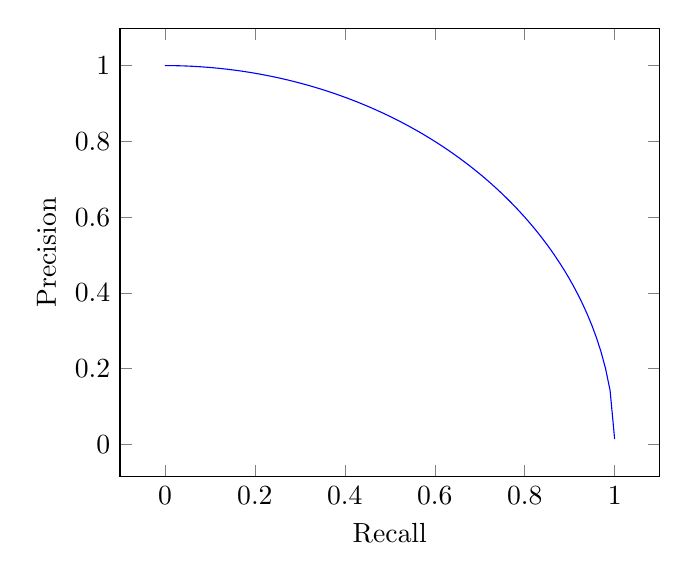
\begin{tikzpicture} []
    \begin{axis}[xlabel = {Recall}, ylabel = {Precision}]
        \addplot [domain = 0:1, samples = 100, blue] {sqrt(1 - x^2)};
    \end{axis}
    \end{tikzpicture}
}
\end{center}
To decide which model to choose, we should look at both precision($P$) and recall($R$). To make the decision easier, we define a new metric called $\mathbf{F_1 score}$ which is a combination of $P$ and $R$ and is defined as follows:
\[F_1 score = \frac{1}{\frac{1}{2}(\frac{1}{P}+\frac{1}{R})} = \frac{2PR}{P+R}\]
Now we can choose the algorithm with the highest $F_1 score$.

\section{Week 4: Decision Trees}

This week, you'll learn about a practical and very commonly used learning algorithm the decision tree. You'll also learn about variations of the decision tree, including random forests and boosted trees (XGBoost).

\subsection{Decision Tree Model}

A decision tree model is a hierarchical, tree structure, which consists of a root node, internal nodes, and leaf nodes. This tree structure helps us to solve both classification and regression problems. In this tree structure, the internal nodes of our tree are called \textbf{decision nodes} which contain the features of our model, and the leaf nodes are called \textbf{terminal nodes} which contain the outputs of our model. For example, suppose we have a cat/dog classification task. In this case, each feature will be assigned to a decision node (i.e. internal node), and each leaf node (i.e. terminal node) will contain either \emph{cat} or \emph{not cat}. Then when a new example is given to our model, we simply start from the root and get to a leaf node, where the decision nodes show the path to follow.

Here, we suppose that each feature is a binary feature (i.e. it gets either 0 or 1). In other cases, we can convert a feature to one or more binary features and continue assuming that all features are binary:

\begin{itemize}
    \item \textbf{Discrete Feature:} If a feature gets $k$ different values, we convert it into $k$ different features and evaluate them using \textbf{one-hot encoding}. For example, suppose that we have the feature \emph{ear shape} which can get three values \emph{pointy}, \emph{oval}, and \emph{floppy}. Then we replace this feature with three new features that are binary and only one of them is 1 at a time (i.e. in a single training example). This is why it is called one-hot encoding.
    \item \textbf{Continuous Feature:} In this case, we set a threshold to convert this feature into a binary feature. For example, if we have the feature \emph{weight} that gets continuous values, we replace it with a binary feature that tells if the weight is less than 5kg or not.
\end{itemize}

\noindent The following figure indicates a simple decision tree for our previous example:

\begin{figure} [h]
    \centering
    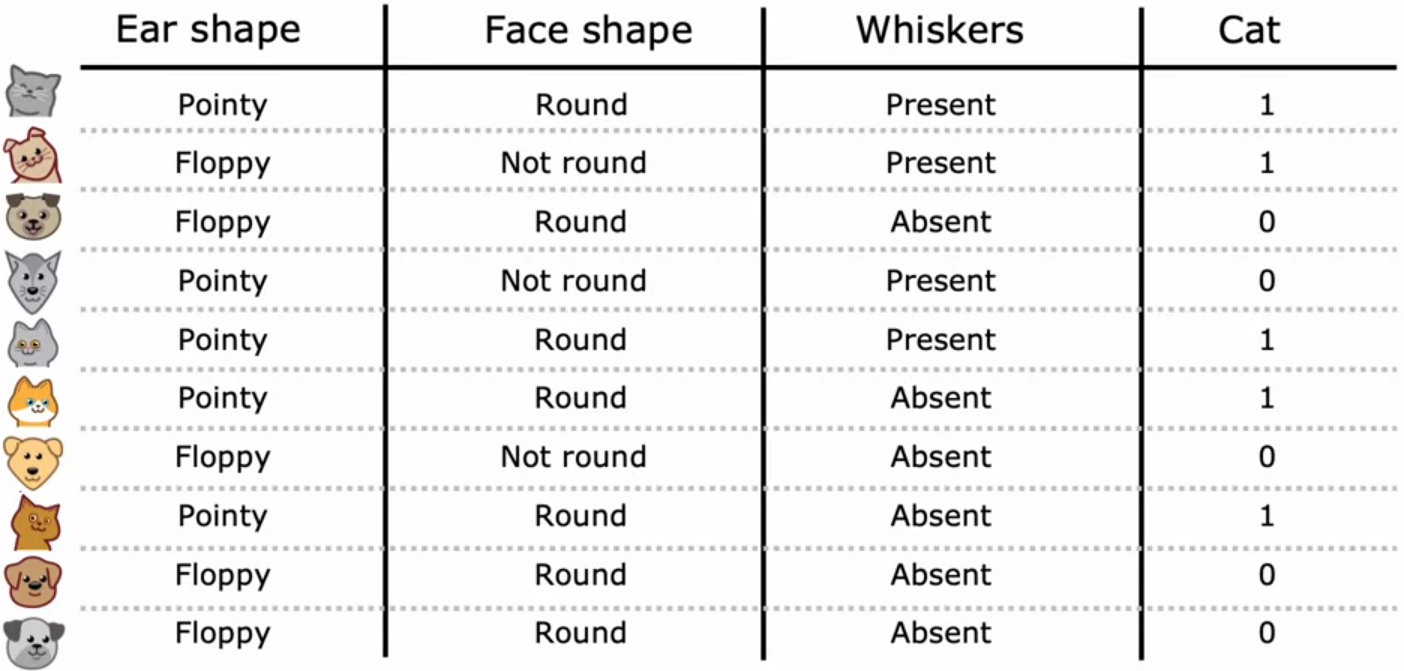
\includegraphics[width=0.55\textwidth]{graphics/sdt_table.png}
    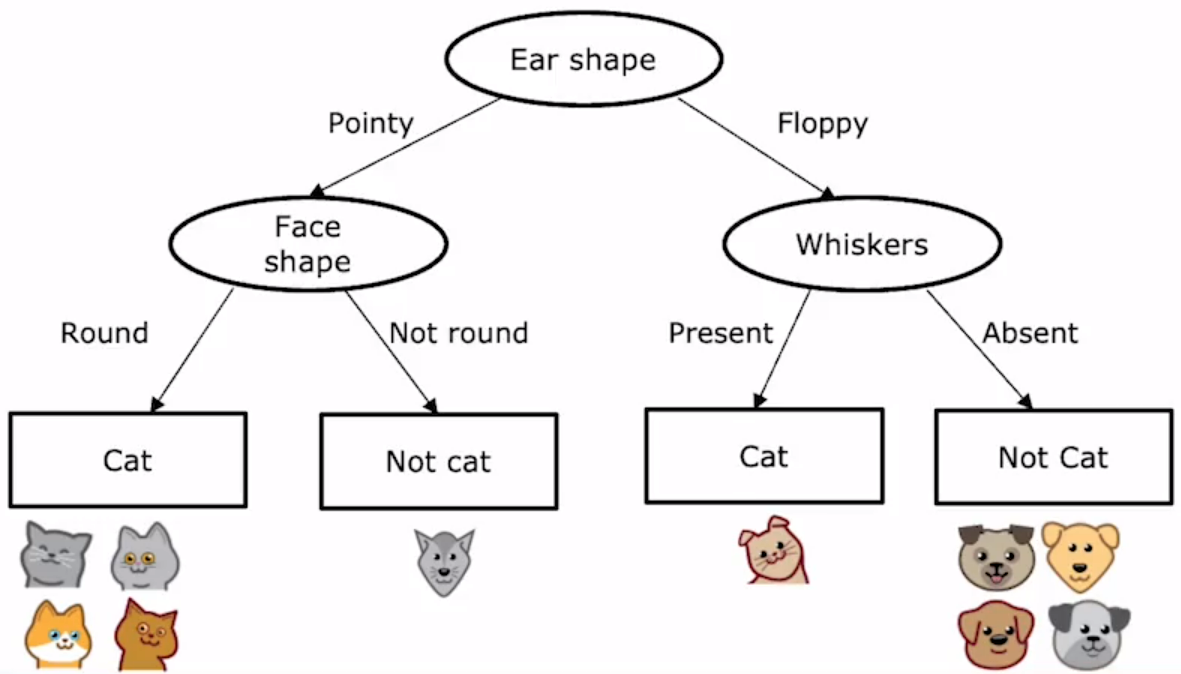
\includegraphics[width=0.4\textwidth]{graphics/simple_dec_tree.png}
    \caption{An example of a simple decision tree for cat/dog classification}
\end{figure}

\subsection{Entropy and Information Gain}

The process of training a decision tree model consists of choosing features assigned to the internal nodes. So, we need a method to decide which feature goes in each decision node. While there are multiple ways to select the best feature at each node, two methods, \textbf{Information Gain}, and \textbf{Gini Impurity}, act as popular splitting criteria for decision tree models. Here, we are going to use the information gain method.

First, notice that the ideal feature for a node is the one that splits our data into two completely pure sets (i.e. all cats and all dogs). But in real-life examples, that is not often the case. So, there is a need to define a function that shows how pure (or impure) a set is. In order to do that, let's introduce the \textbf{Entropy} function which gets a set and measures its impurity: \[H(S) = -\sum_{c \in C} p_c \log_2(p_c)\] where $S$ is the data set that entropy is calculated, $c$ represents the classes in $S$, and $p_c$ represents the proportion of data points that belong to class c to the number of total data points in $S$. In our classification problem where there are only two classes, the entropy function is like this:
\[H(p_1) = -p_1 \log_2(p_1) - (1 - p_1) \log_2(1- p_1)\] where $p_1$ is the proportion of cats in the set. The plot of the entropy function is as follows:

\begin{center}
    \resizebox{0.4\textwidth}{!}{
        \begin{tikzpicture} []
        \begin{axis}[xlabel = {$p_1$},
                    ylabel = {$H(p_1)$}]
            \addplot [domain = 0:1, samples = 100, red] {-x*log2(x) - (1-x)*log2(1-x)};
        \end{axis}
        \end{tikzpicture}
    }
\end{center}

Note that the entropy function reaches its highest value (1) when $p_1 = 0.5$, which means the set is completely impure. Also note that when $p_1 = 1$ or $0$, the entropy is $0$, which means the set is completely pure. When we split a set at a node according to a specific feature, we come up with two new entropy values for the left and right branches. To be able to decide based on these values, we define a new function called \textbf{Information Gain} which shows how much the entropy has decreased by splitting a set. \[\text{Information Gain} = H(p_1^\text{node})- \left(w^{\text{left}}H(p_1^\text{left}) + w^{\text{right}}H(p_1^\text{right})\right)\] where $w^{\text{left}}$ and $w^{\text{right}}$ are the proportions of new sets after we split the old set (note that $w^{\text{left}} + w^{\text{right}} = 1$). In a more general form, the information gain function is defined as follows: \[\text{Gain}(S, a) = H(S) - \sum_{v \in \text{Values}(a)} \frac{|S_v|}{|S|}H(S_v)\] where $a$ is the feature and $S_v$ represents each new set.

Now that we have defined the information gain function, we can finally decide which feature to put in a node. The following algorithm is a recursive algorithm (similar to DFS) by which we can build a decision tree:

\begin{algorithm}
\caption{Build a Decision Tree Model}
\begin{algorithmic} [1]
\Procedure{BuildDecisionTree}{$Tree$, $Node$, $DataSet$}
  \If{\Call{BaseCondition}{$Tree$, $Node$, $DataSet$}}
    \State Evaluate as a Leaf Node
    \State \Return
  \EndIf
  \State $\text{BestFeature} \gets \arg \max \bigl[\Call{InformationGain}{DataSet, \text{feature}}\bigr]$
  \State $\text{LeftBranch}, \text{RightBranch} \gets \Call{Split}{\text{BestFeature}, DataSet}$
  \State $\Call{BuildDecisionTree}{Tree, Node.\text{left}, \text{LeftBranch}}$
  \State $\Call{BuildDecisionTree}{Tree, Node.\text{right}, \text{RightBranch}}$
\EndProcedure
\State 
\State $Tree \gets \Call{NewTree}$
\State $\Call{BuildDecisionTree}{Tree, Tree.\text{root}, DataSet}$
\end{algorithmic}
\end{algorithm}

\noindent where the $\Call{BaseCondition}$ checks for one of the following conditions:

\begin{itemize}
    \item If the node is 100\% one class
    \item If splitting a node results in the tree exceeding a maximum depth
    \item If the information gain from additional splits is less than a threshold
    \item If the number of examples in the node is less than a threshold
\end{itemize}

\noindent So far, you can solve classification problems with decision trees. In order to solve regression problems, all we have to do is to replace entropy with \textbf{variance}. And also when we reach a leaf node, we report the \textbf{mean} of the examples to make regression predictions.

\subsection{Tree Ensembles}

It turns out that while using a single decision tree to make predictions, a single change in training examples will cause many changes in the whole tree structure. So, in order to solve this problem, researchers have come up with the idea of \textbf{tree ensembles}. The intuition behind tree ensembles is that instead of using only a single decision tree, we use a bunch of different ones. Then in the inference stage, we let each decision tree vote and we report the result according to that (or in regression tasks, we could report the mean of trees).

In order to build a tree ensemble, we use a process called \textbf{random sampling with replacement} came from statistics. The following algorithm shows how we can build a tree ensemble (also called \textbf{random forest}):

\begin{algorithm}
\caption{Build a Random Forest}
\begin{algorithmic} [1]
\Require $\text{Training set of size} m$
\State $\text{ensemble} \gets \Call{NewSet}$
\For{$b=1$ to $B$}
    \State $\text{newTrainingData} \gets \Call{SampleWithReplacement}{TrainingSet, m}$
    \State $\text{newDecisionTree} \gets \Call{BuildDecisionTree}{\text{newTrainingData}}$ 
    \State $\text{ensemble.}\Call{Append}{\text{newDecisionTree}}$
\EndFor
\end{algorithmic}
\end{algorithm}

It turns out that even though we sample randomly each time, in so many cases there is no change in the features selected for the root node and nodes in the first few layers. In order to solve this problem, at each node, when choosing a feature to use to split, if $n$ features are available, we pick a random subset of $k < n$ features and allow the algorithm to only choose from that subset of features (a common choice is to set $k = \sqrt{n}$).

\subsection{XGBoost (Extreme Gradient Boosting)}

The boosting methods train several trees, but instead of them being uncorrelated to each other, now the trees fit one after the other in order to minimize the error. The main difference the \textbf{XGBoost} algorithm has is in the sampling step. In this algorithm, instead of picking from all examples with equal probability ($\frac{1}{m}$), we make it more likely to pick misclassified examples from previously trained trees.

The XGBoost algorithm is an open-source, fast, and efficient implementation of boosted trees and is highly used in machine learning competitions. It also implements a good choice of default splitting criteria and criteria for when to stop splitting. In addition, it has a built-in regularization to prevent overfitting. You can simply use the XGBoost algorithm using open-source libraries:

\begin{table}[h]
\noindent\begin{minipage}{.45\textwidth}
\begin{lstlisting}[language=Python, caption={XGBoost for Classification}]
from xgboost import XGBClassifier

model = XGBClassifier()

model.fit(X_train, y_train)
y_pred = model.predict(X_test)
\end{lstlisting}
\end{minipage}\hfill
\noindent\begin{minipage}{.45\textwidth}
\begin{lstlisting}[language=Python, caption={XGBoost for Regression}]
from xgboost import XGBRegressor

model = XGBRegressor()

model.fit(X_train, y_train)
y_pred = model.predict(X_test)
\end{lstlisting}
\end{minipage}
\end{table}

\subsection{Decision Trees vs. Neural Networks}

The following table shows the differences between decision trees and neural networks. It will help you to decide which one to pick for your machine learning tasks:

\begin{center}
\begin{tabular}{ |c|c| } 
 \hline
 \textbf{Decision Trees and Tree Ensembles} & \textbf{Neural Networks} \\
 \hline
 works well on tabular (structured) data & works well on all types of data \\ 
 fast in training and inference & may be slower than a decision tree\\ 
 not compatible with transfer learning & works with transfer learning \\ 
 small decision trees may be human readable & easy to string together to build large systems \\ 
 \hline
\end{tabular}
\end{center}

\chapter{Unsupervised Learning}

\section{Week 1: Clustering and Anomaly Detection}

\subsection{Clustering Intuition}

Clustering is an unsupervised learning task that aims to divide unlabeled data into different groups. In mathematical terms, we have $m$ points in $n$-dimensional space and the task is to put these points in $K$ clusters (groups) in a way that points in each cluster are relevant to each other. In the following section, we will introduce an algorithm called \textbf{K-means Clustering} to perform clustering tasks.

\subsection{K-means Clustering Algorithm}

In this algorithm, we use an auxiliary point called \textbf{cluster centroid} for each cluster. At each step of the algorithm, we assign points to their closest centroid and then move each centroid to its new position which is the mean of the points assigned to it. Let's define some symbols:

\begin{itemize}
    \item $c^{(i)}$: index of cluster to which example $x^{(i)}$ is currently assigned
    \item $\mu_k$: cluster centroid $k$
    \item $\mu_{c^{(i)}}$: cluster centroid of cluster to which example $x^{(i)}$ has been assigned
\end{itemize}

\noindent Now we can write the algorithm in mathematical terms:

\begin{algorithm} [h]
\caption{K-means Clustering}
\begin{algorithmic} [1]
\State $\mu \gets \Call{RandomPoints}{K}$
\State $c \gets \Call{EmptyArray}{m}$
\Repeat
    \For{$i=1$ to $m$}
        \State $c^{(i)} \gets \Call{ClosestClusterCentroid}{\mu}$
    \EndFor
    \For{$k=1$ to $K$}
        \State pointsAssignedToClusterK $\gets$ X[c == k]
        \State $\mu_k \gets \Call{Mean}{\text{pointsAssignedToClusterK}}$
    \EndFor
\Until{the algorithm converges}

\end{algorithmic}
\end{algorithm}

It is common to instead of choosing completely random points in $\Call{RandomPoints}$, we choose some of the training examples randomly as starting points for cluster centroids. It is also common that when a cluster centroid gets assigned by no points (in line 7), we eliminate that cluster and continue the algorithm with $K-1$ clusters. Another thing we can do is restart the algorithm with different random initial centroids, but this approach is not that common.

\subsubsection{Distortion Function for K-means Clustering}

In each iteration of the K-means algorithm, we are trying to minimize a cost function called \textbf{distortion function} and is defined as follows: \[J(c,\mu) = \frac{1}{m}\sum_{i=1}^m \|x^{(i)} - \mu_{c^{(i)}}\|^2\] It turns out that choosing different initial centroids will cause significant changes in our final clustering model. Thus, it is common to run the algorithm multiple times and pick the one that gave the lowest distortion function.

\subsubsection{Choosing Number of Clusters}

The number of clusters ($K$) highly depends on the underlying purpose of the clustering task. But if we have no prior knowledge about the number of clusters, there is a method called \textbf{elbow} to help us choose the right value for $K$. In this method, we calculate the cost function (distortion) for each value of $K$ and if we can find an elbow shape in the plot, we choose that value as $K$. The following plot shows what we mean by an elbow shape:

\begin{center}
    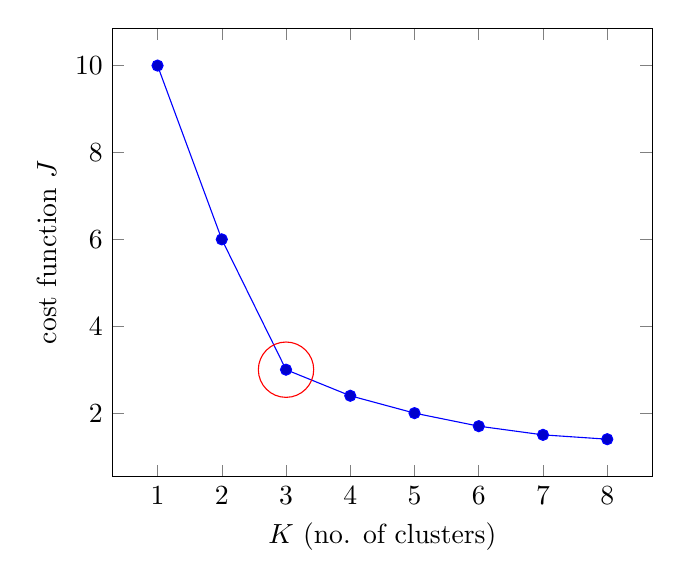
\begin{tikzpicture}
        \begin{axis}[
            xlabel = {$K$ (no. of clusters)},
            ylabel = {cost function $J$},
            xtick={1,2,...,8}]
        
            \addplot+ [mark=*] table {
            1  10
            2  6
            3  3
            4  2.4
            5  2
            6  1.7
            7  1.5
            8  1.4
            };

            \addplot+ [mark=o, mark size=10pt] table {
            3  3
            };
        \end{axis}
\end{tikzpicture}
\end{center}

In the above plot, there is an elbow shape at point $(3,3)$, so we prefer to use $K=3$ as the number of clusters. Note that we cannot choose a $K$ that minimizes the cost function, because $J(\mu,c)$ is a decreasing function.
\newpage

\subsection{Anomaly Detection}

Anomaly detection is when our model is shown a number of normal examples and it aims to detect anomalies in new examples. For example, if we want to detect fraud activities of users on a website, we can use an anomaly detection model and use the number of logins and requests of a user as features.

The main idea is to fit a probability distribution to our data. In more precise terms, we define a joint probability density function (PDF) in terms of our features (features as random variables). We often use a normal distribution with parameters $\mu$ and $\sigma^2$ to fit into our data. Assuming that our features are independent random variables $X_1$, $X_2$, ..., $X_n$, we can say:
\[f_{X_1 X_2 \dots X_3}(x_1, x_2, \dots, x_n) = f_{X_1}(x_1) f_{X_2}(x_2) \dots f_{X_n}(x_n)\]
So we only need to fit a normal distribution into each of our features independently. In order to build normal distributions, we use two estimators\footnote{These estimators are derived from \emph{maximum likelihood estimator (MLE)} method.} for $\mu$ and $\sigma^2$:
\[\mu_j = \frac{1}{m} \sum_{i=1}^m x_j^{(i)} \qquad \qquad \sigma_j^2 = \frac{1}{m} \sum_{i=1}^m (x_j^{(i)} - \mu_j)^2 \]
And so the marginal probability of $X_j$ is calculated as follows:
\[f_{X_j}(x_j) = p(x_j;\mu_j,\sigma_j^2) = \frac{1}{\sqrt{2\pi\sigma_j^2}} \exp\left(-\frac{(x_j - \mu_j)^2}{2\sigma_j^2}\right)\]
Then we can define our model as the joint probability density function:
\[p(\Vec{x}) = p(x_1;\mu_1,\sigma_1^2) p(x_2;\mu_2,\sigma_2^2) \dots p(x_n;\mu_n,\sigma_n^2) = \prod_{j=1}^np(x_j;\mu_j,\sigma_j^2)\]
Now in the inference phase, when we are given a new example $\Vec{x}$, we calculate $p(\Vec{x})$ and based on the obtained probability, we can decide if it is a normal example or is an anomalous one.
\[y = \begin{cases}
    1 \quad \text{if } p(x) < \epsilon \text{ (anomaly)} \\
    0 \quad \text{if } p(x) \geq \epsilon \text{ (normal)} \\
\end{cases}\]
For example, if we have 2 features and the following points (normal examples):

\begin{center}
  \centering
  \begin{tikzpicture}
    \begin{axis}[
      xlabel={$x_1$},
      ylabel={$x_2$}]
      \addplot [only marks, mark=*, mark size=3, scatter] table[col sep=comma, x=x1, y=x2] {data/anomaly.csv};
    \end{axis}
  \end{tikzpicture}
\end{center}

Then we can fit the following joint normal distribution with parameters $\mu_1 = 5, \sigma_1 = 2$ and $\mu_2 = 3, \sigma_2 = 1$:

\begin{center}
  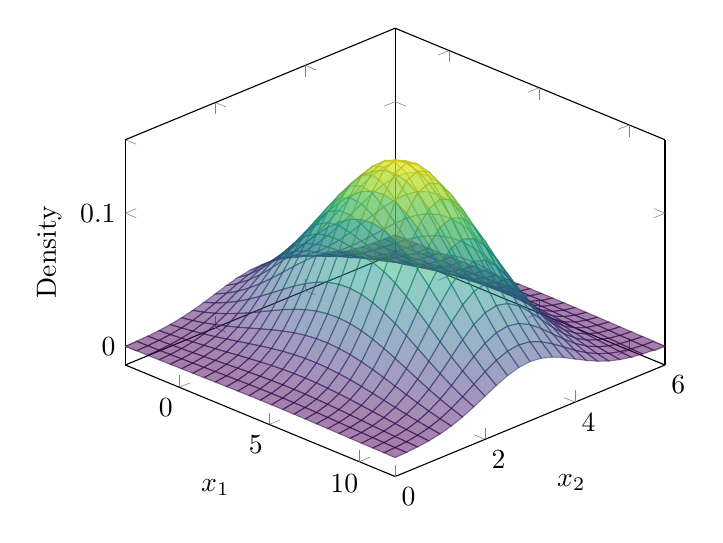
\begin{tikzpicture}
    \begin{axis}[
      view={45}{35}, % Set the viewing angle
      xlabel={$x_1$},
      ylabel={$x_2$},
      zlabel={Density}]
      \addplot3[surf, opacity=0.5, domain=-3:12, domain y=0:6, colormap/viridis] {1/(4*sqrt(pi)) * e^(-(((y-3)^2)/2 + ((x-5)^2)/32))};
    \end{axis}
  \end{tikzpicture}
\end{center}

You can see both the training examples and the Gaussian distribution in the following contour plot:

\begin{center}
  \centering
  \begin{tikzpicture}
    \begin{axis}[
      xlabel={$x_1$},
      ylabel={$x_2$},
      view={0}{90}]
      \addplot [only marks, mark=*, mark size=3, scatter] table[col sep=comma, x=x1, y=x2] {data/anomaly.csv};
      \addplot3[contour gnuplot={levels={0.02,0.04,0.06,0.08,0.1,0.12}, labels=false}, thick, domain=0:11, domain y=0:7, colormap/viridis] {1/(4*sqrt(pi)) * e^(-(((y-3)^2)/2 + ((x-5)^2)/32))};
    \end{axis}
  \end{tikzpicture}
\end{center}

\subsubsection{Algorithm Evaluation}

In anomaly detection tasks, we often have a large number of unlabeled examples (but we know that most of them are normal). In order to evaluate our model, we need some labeled examples to put in cross-validation and test sets. Then we can use evaluation metrics like precision, recall, and $F_1$-score. It is common to use the cross-validation set to choose parameter $\epsilon$ and then use the test set to evaluate the model.

\subsubsection{Error Analysis for Anomaly Detection}

The most common bug in anomaly detection models is that $p(x)$ is large for both normal and anomalous examples. This problem usually means that the features we have chosen, are not able to clearly specify the anomaly in the system. In this case, we often add other features that may be relevant to anomalous behavior in data.
\newpage

For instance, suppose we want to monitor computers in a data center and we have the following features:

\begin{itemize}
    \item $x_1$ = memory use of computer
    \item $x_2$ = number of disk accesses/sec
    \item $x_3$ = CPU load
    \item $x_4$ = network traffic
\end{itemize}

\noindent Then adding the following features will cause small values for $p(x)$ for anomalous $x$ in the cross-validation set:
\[ x_5 = \frac{x_3}{x_4} \qquad x_6 = \frac{(x_3)^2}{x_4} \]
The other common problem in anomaly detection systems occurs when our features are non-gaussian and thus we can not efficiently fit a normal distribution into it. In order to make the variables more like Gaussian distribution, it is recommended to apply one of the following operations to the features:
\[x \gets log(x) \qquad x \gets log(x + c) \qquad x \gets \sqrt{x} \qquad x \gets x^{\frac{1}{3}} \]

\subsection{Anomaly Detection vs. Supervised Learning}

In most cases, when we have an anomaly detection task, we can think about supervised learning algorithms too. In the table below, there are some tips to help you choose what approach should you take.

\begin{center}
\begin{tabular}{| p{0.43\linewidth} | p{0.43\linewidth} |}
 \hline
 \centering \textbf{ Anomaly Detection} & \centering \textbf{Supervised Learning} \tabularnewline
 \hline
 Very small number of positive examples (0-20 is common). Large number of negative examples & Large number of positive and negative examples \\ 
 Many different types of anomalies. Hard for any algorithm to learn from positive examples what the anomalies look like; future anomalies may look nothing like any of the anomalous examples we have seen so far. & Enough positive examples for the algorithm to get a sense of what positive examples are like; future positive examples are likely to be similar to ones in the training set.\\ 
 \hline
\end{tabular}
\end{center}

\noindent Examples of each one:

\begin{center}
\begin{tabular}{|c|c|}
 \hline
 \textbf{Anomaly Detection} & \textbf{Supervised Learning} \\
 \hline
 Fraud detection & Email spam classification \\ 
 Finding new previously unseen defects & Finding known, previously seen defects\\
 Aircraft engines defect detection & Weather prediction \\
 Monitoring machines in a data center & Diseases classification \\
 \hline
\end{tabular}
\end{center}

\section{Week 2: Recommender Systems}

\subsection{Collaborative Filtering}
Suppose there is a movie website that has the data of ratings of users given to different movies. If we denote the number of users and the number of movies by $n_u$ and $n_m$ respectively, our data of ratings (from zero to five) can be shown by the following matrix:
\[
\mathbf{Y} = \begin{bmatrix}
    4 & 5 & \dots & 2.5\\
    3.5 & ? & \dots & 0 \\
    \vdots & \vdots & \ddots & \vdots \\
    ? & 0.5 & \dots & 4.5
\end{bmatrix}_{n_m\times n_u}
\]
The columns are users and rows are movies, So $y^{(i,j)}$ is the rating given by user $j$ to movie $i$. The $\mathbf{?}$ signs in the matrix $Y$ show that the user has not rated a movie so far. We can define the following matrix that indicates if a user has rated for a movie or not:
\[
\mathbf{R} = \begin{bmatrix}
    1 & 1 & \dots & 1\\
    1 & 0 & \dots & 1 \\
    \vdots & \vdots & \ddots & \vdots \\
    0 & 1 & \dots & 1
\end{bmatrix}_{n_m\times n_u}
\]
Suppose we have features of the movies (number of features = $n$). For example, if $x_1$ is the amount of romance and $x_2$ is the amount of action, ... then We can show the features using the following matrix:
\[
\mathbf{X} = \begin{bmatrix}
    0.9 & 0.0 & \dots & 0.2\\
    1.0 & 0.01 & \dots & 0.7 \\
    \vdots & \vdots & \ddots & \vdots \\
    0.1 & 0.99 & \dots & 0.0
\end{bmatrix}_{n_m\times n}
\]
In the case that we have the features of each movie (we are given the matrix $X$), we can predict user $j$'s rating for movie $i$ as \[\mathbf{w}^{(j)} \cdot \mathbf{x}^{(i)} + b^{(j)}\] In this case, we are fitting a linear regression model for each user separately. So the cost function for user $j$ is \[J(\mathbf{w}^{(j)}, b^{(j)}) = \frac{1}{2}\sum_{i:R_{ij}=1} (\mathbf{w}^{(j)} \cdot \mathbf{x}^{(i)} + b^{(j)} - y^{(i,j)})^2 + \frac{\lambda}{2}\sum_{k=1}^{n}(\mathbf{w}^{(j)}_k)^2\]
And for all users:
\[J(\mathbf{W}, \mathbf{b}) = \sum_{j=1}^{n_u} J(\mathbf{w}^{(j)}, b^{(j)})\]
In real-life situations, we often do not have the features of each movie. Now imagine that we are given the features $\mathbf{W}$ and $\mathbf{b}$. Now the cost function for feature $x^{(i)}$ is defined as follows:
\[ J(x^{(i)}) = \frac{1}{2}\sum_{j:R_{ij}=1} (\mathbf{w}^{(j)} \cdot \mathbf{x}^{(i)} + b^{(j)} - y^{(i,j)})^2 + \frac{\lambda}{2}\sum_{k=1}^{n}(\mathbf{x}^{(j)}_k)^2 \]
And for all features:
\[ J(\mathbf{X}) = \sum_{j=1}^{n_m} J(\mathbf{w}^{(j)}, b^{(j)}) \]
Now in the case where we have neither features nor parameters, we can put the two equations together and come up with the following cost function:
\[ J(\mathbf{X},\mathbf{W},\mathbf{b}) = \left[ \frac{1}{2}\sum_{(i,j):R_{ij}=1}(\mathbf{w}^{(j)} \cdot \mathbf{x}^{(i)} + b^{(j)} - y^{(i,j)})^2 \right]
+ \underbrace{\left[
\frac{\lambda}{2}
\sum_{j=1}^{n_u}\sum_{k=1}^{n}(\mathbf{w}^{(j)}_k)^2
+ \frac{\lambda}{2}\sum_{i=1}^{n_m}\sum_{k=1}^{n}(\mathbf{x}_k^{(i)})^2
\right]}_{regularization} \]
Then we can use gradient descent to find the minimum point of $J(\mathbf{X},\mathbf{W},\mathbf{b})$ with the difference that here $\mathbf{X}$ is also a parameter as well as $\mathbf{W}$ and $\mathbf{b}$. So in each iteration of gradient descent, we now have an extra term for $\mathbf{X}$ and our algorithm is turned to this:

\begin{algorithm}
\caption{Gradient Descent Algorithm for Collaborative Filtering}
\begin{algorithmic} [1]
\Repeat
    \State $w^{(j)}_i \gets w^{(j)}_i - \alpha{\frac{\partial}{\partial w^{(j)}_i}}J(w,b,x)$
    \State $b^{(j)} \gets b^{(j)} - \alpha{\frac{\partial}{\partial b^{(j)}}}J(w,b,x)$
    \State $x^{(i)}_k \gets x^{(i)}_k - \alpha{\frac{\partial}{\partial x^{(i)}_k}}J(w,b,x)$
\Until{convergence}
\end{algorithmic}
\end{algorithm}

\subsubsection{Collaborative Filtering for Binary Labels}

There are lots of times when our data is binary in recommender systems. For example, a user can like/dislike a post on social media, or a user can purchase or don't purchase a specific commodity on an online shop. In these cases, we use the logistic function (with analogy to when we moved from regression to classification). In more concrete terms, we predict that the probability of $y^{(i,j)} = 1$ is given by \[f_{w,b,x}(\mathbf{x}) = g(\mathbf{w}^{(j)} \cdot \mathbf{x}^{(i)} + b^{(j)}), \qquad \text{where} \quad g(z) = \frac{1}{1+e^{-z}}\]
In addition to our model function, the cost function also changes. The loss function for a single example is as follows:
\[ L(f_{w,b,x}(x), y^{(i,j)}) = -y^{(i,j)} \log (f_{w,b,x}(x)) - (1 - y^{(i,j)})\log(1 - f_{w,b,x}(x)) \]
And the cost function for all examples is
\[J(\mathbf{W}, \mathbf{b}, \mathbf{X}) = \sum_{(i,j):R_{ij}=1} L(f_{w,b,x}(x), y^{(i,j)})\]

\subsection{Recommender Systems Implementation Details}

With our model so far, if a new user register to our website and has not rated any movies yet, our model will predict that they will rate zero to all movies. In order to fix that problem, we use a method called \textbf{Mean Normalization} in which we calculate the mean of each row in matrix $\mathbf{Y}$ and store them in a vector like $\mu$. Then we subtract each it from each row of $\mathbf{Y}$: \[Y_j = Y_j - \mu\] Then we define our model function to be \[f_{w,b,x}(x) = \mathbf{w}^{(j)} \cdot \mathbf{x}^{(i)} + b^{(j)} + \mu_i\] This will fix the problem because now a new user will be assigned with average ratings of other users for movies.

\subsubsection{Finding Related Items}

When we are using collaborative filtering, we often cannot interpret the features $\mathbf{x}^{(i)}$ of item $i$ (features do not represent something specific like genre). So, to find other items related to an item, we can find the nearest item (say $k$) in the Euclidean space in a way that the Euclidean distance between $\mathbf{x}^{(i)}$ and $\mathbf{x}^{(k)}$ is minimum: $\| \mathbf{x}^{(k)} - \mathbf{x}^{(i)} \|^2$

\subsection{TensorFlow Implementation of Collaborative Filtering}

TensorFlow enables us to run gradient descent in whatever cost function we want. We just need to define the cost function and let TensorFlow compute the partial derivatives. We can also customize the optimizer we want to use. The following code indicates how to use a predefined cost function and run gradient descent with Adam optimizer:

\begin{lstlisting}[language=Python]
# Set Initial Parameters (W, X), use tf.Variable to track these variables
tf.random.set_seed(1234) # for consistent results
W = tf.Variable(tf.random.normal((num_users,num_features)), name='W')
X = tf.Variable(tf.random.normal((num_movies, num_features)), name='X')
b = tf.Variable(tf.random.normal((1, num_users)), name='b')

# Instantiate an optimizer.
optimizer = keras.optimizers.Adam(learning_rate=1e-1)

iterations = 200
lambda_ = 1
for it in range(iterations):
    # Use TensorFlow's GradientTape
    # to record the operations used to compute the cost 
    with tf.GradientTape() as tape:

        # Compute the cost (forward pass included in cost)
        cost_value = cofi_cost_func_v(X, W, b, Ynorm, R, lambda_)

    # Use the gradient tape to automatically retrieve
    # the gradients of the trainable variables with respect to the loss
    grads = tape.gradient( cost_value, [X,W,b] )

    # Run one step of gradient descent by updating
    # the value of the variables to minimize the loss.
    optimizer.apply_gradients( zip(grads, [X,W,b]) )
\end{lstlisting}

\subsection{Limitations of Collaborative Filtering}

Collaborative filtering has two major limitations:

\begin{enumerate}
    \item Cold start problem:
        \begin{itemize}
            \item How to rank new items that few users have rated?
            \item How to show something reasonable to new users who have rated few items?
        \end{itemize}
    \item Use side information about items or users:
        \begin{itemize}
            \item Item: genre, movie stars, studio, ...
            \item User: demographics (age, gender, location), expressed preferences
        \end{itemize}
\end{enumerate}

\subsection{Content-based Filtering}

Previously in collaborative filtering, items are recommended to you based on ratings of users who gave similar ratings as you. In content-based filtering, there are features for users too; and items are recommended to you based on features of user and item to find good match.

We denote features of user $j$ by $x_u^{(j)}$ and features of movie $i$ by $x_m^{(i)}$. Note that these two vectors could be of different dimension (number of user features are often much more). For example, user features could be age, gender, country (one-hot, 200 new features), average rating per genre, etc. and movie features could be year, genre, reviews, average rating, etc.

In content-based filtering, the rating of user $j$ on movie $i$ is predicted as \[\text{Prediction:} \quad v_u^{(j)} \cdot v_m^{(i)}\] Where $v_u^{(j)}$ is computed from $x_u^{(j)}$ and $v_m^{(i)}$ is computed from $x_m^{(i)}$. Note that in order to be able to perform dot product, the dimensions has to be the same, thus $v_u^{(j)}$ and $v_m^{(i)}$ have the same number of elements. The idea is to use two neural networks with same number of elements in output layer to compute $v_u^{(j)}$ and $v_m^{(i)}$. Then we connect these neural networks using a node that perform dot product:
\begin{center}
    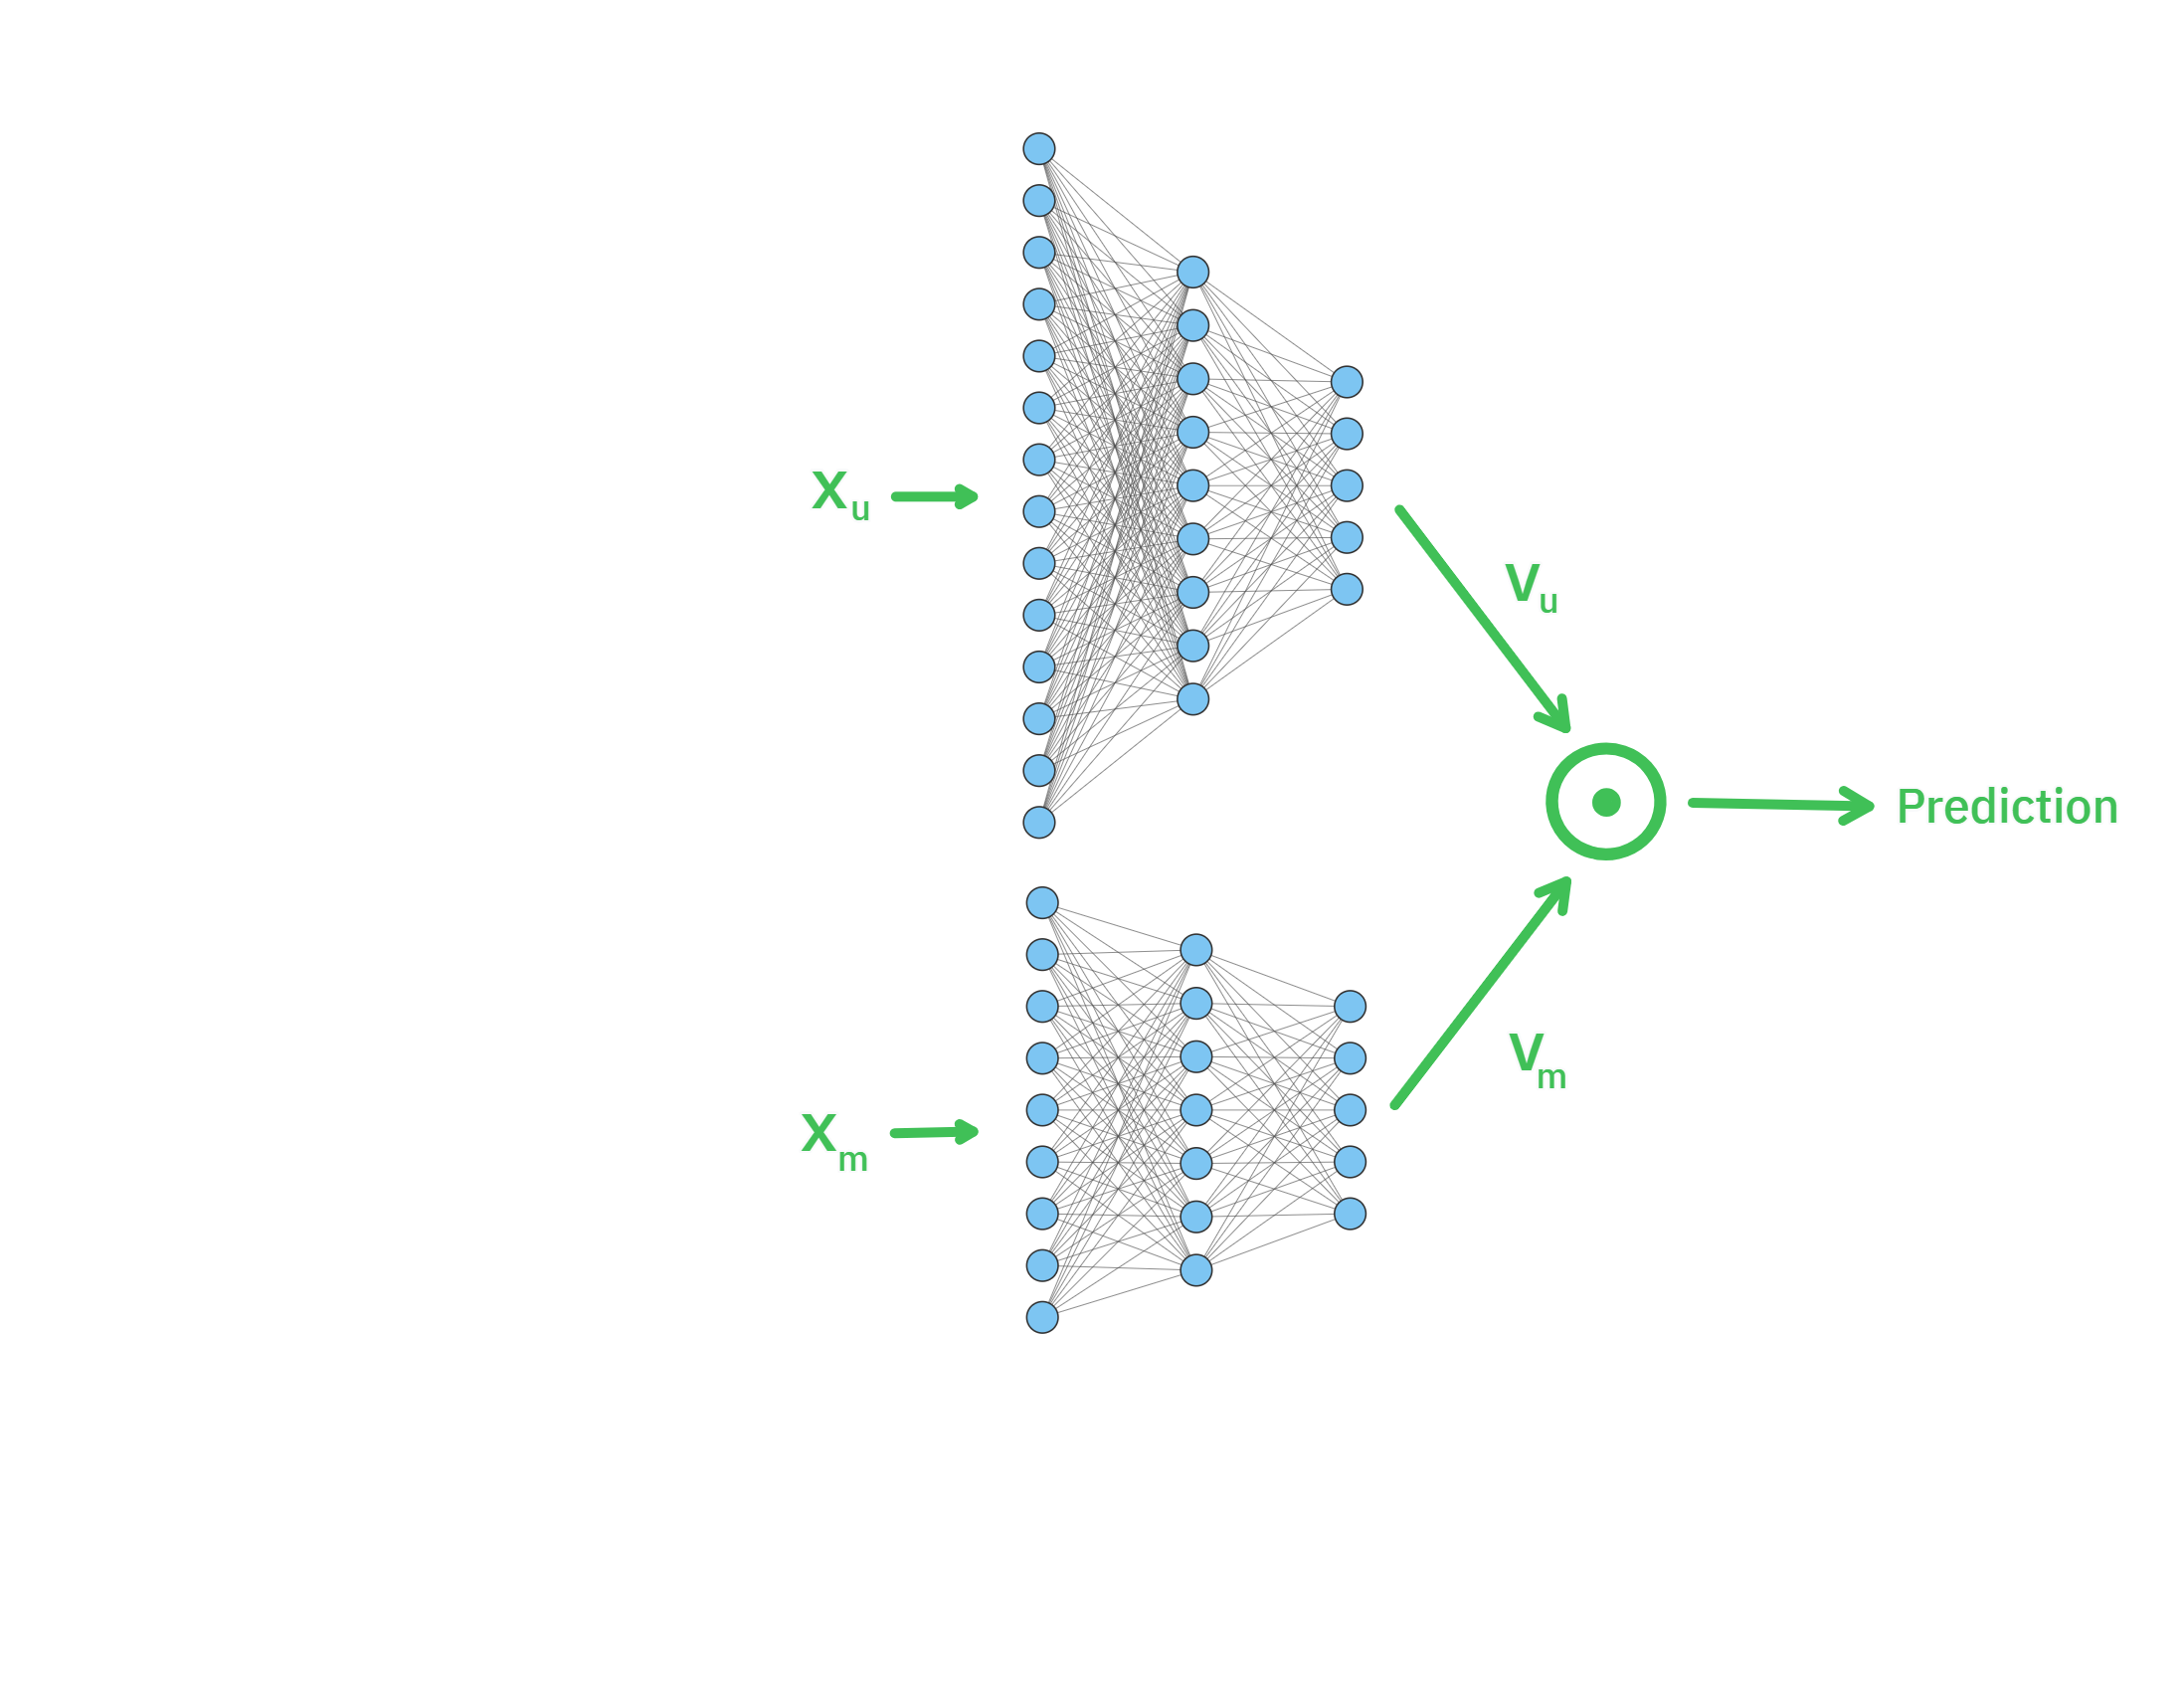
\includegraphics[width=0.65\textwidth, trim={14cm 8cm 2cm 2cm}]{graphics/contentbased.png}
\end{center}

The cost function in content-based filtering is defined as \[J = \sum_{(i,j): R_{ij}=1} (v_u^{(j)}\cdot v_m^{(i)} - y^{(i,j)})^2 + \text{NN regularization term}\] After we trained our neural network, if we want to find movies similar to movie $i$ we should find $k$ that minimizes $\| v_m^{(k)} - v_m^{(i)} \|^2$. Note that this can be pre-computed ahead of time.

\subsection{TensorFlow Implementation of Content-based Filtering}

Here it comes the content-based filtering implementation in code using TensorFlow:

\begin{lstlisting}[language=Python]
num_outputs = 32
tf.random.set_seed(1)
user_NN = tf.keras.models.Sequential([
    tf.keras.layers.Dense(256, activation='relu'),
    tf.keras.layers.Dense(128, activation='relu'),
    tf.keras.layers.Dense(num_outputs)
])
item_NN = tf.keras.models.Sequential([   
    tf.keras.layers.Dense(128, activation='relu'),
    tf.keras.layers.Dense(64, activation='relu'),
    tf.keras.layers.Dense(num_outputs)
])
# create the user and item input and point to the base network
input_user = tf.keras.layers.Input(shape=(num_user_features))
vu = user_NN(input_user)
vu = tf.linalg.l2_normalize(vu, axis=1)
input_item = tf.keras.layers.Input(shape=(num_item_features))
vm = item_NN(input_item)
vm = tf.linalg.l2_normalize(vm, axis=1)
# compute the dot product of the two vectors vu and vm
output = tf.keras.layers.Dot(axes=1)([vu, vm])
# specify the inputs and output of the model
model = tf.keras.Model([input_user, input_item], output)
\end{lstlisting}

\subsection{Retrieval and Ranking}
Real-world recommendation systems work with millions of users and billions of items. To handle this massive scale, recommendation systems tend to be divided into two types of models (retrieval and ranking), running one after the other, narrowing down the set of items each time:

\begin{enumerate}
    \item Retrieval:
    \begin{itemize}
        \item Generate large list of plausible item candidates. For example:
        \begin{enumerate}
            \item For each of the last 10 movies watched by the user, find 10 most similar movies
            \item For most viewed 3 genres, find the top 10 movies
            \item Top 20 movies in the user's country
        \end{enumerate}
        \item Combine retrieved items into list, removing duplicates and items already watched
    \end{itemize}
    \item Ranking:
    \begin{itemize}
        \item Take list retrieved and rank using learned model
        \item Display ranked items to user
    \end{itemize}
\end{enumerate}

Retrieving more items in the first step results in better performance, but slower recommendations. To analyse and optimize the trade-off, carry out offline experiments to see if retrieving additional items results in more relevant recommendations.

\subsection{Principal Component Analysis}

PCA is a statistical procedure for dimensionality reduction. We are not covering the theory of PCA here. We use PCA to reduce the dimensionality of our data in order to improve interpretablity of data (e.g. demonstrate graphically) or to reduce the size of hardware storage needed for the data.

Suppose we have two parameters \emph{length} and \emph{height} for a car (See figure below). We know that these two features are not independent and are correlated in a direct way. PCA will choose a new axis that can represent each point with a single number without losing much information. This new axis could indicate the \emph{size} of the car.

\begin{center}
    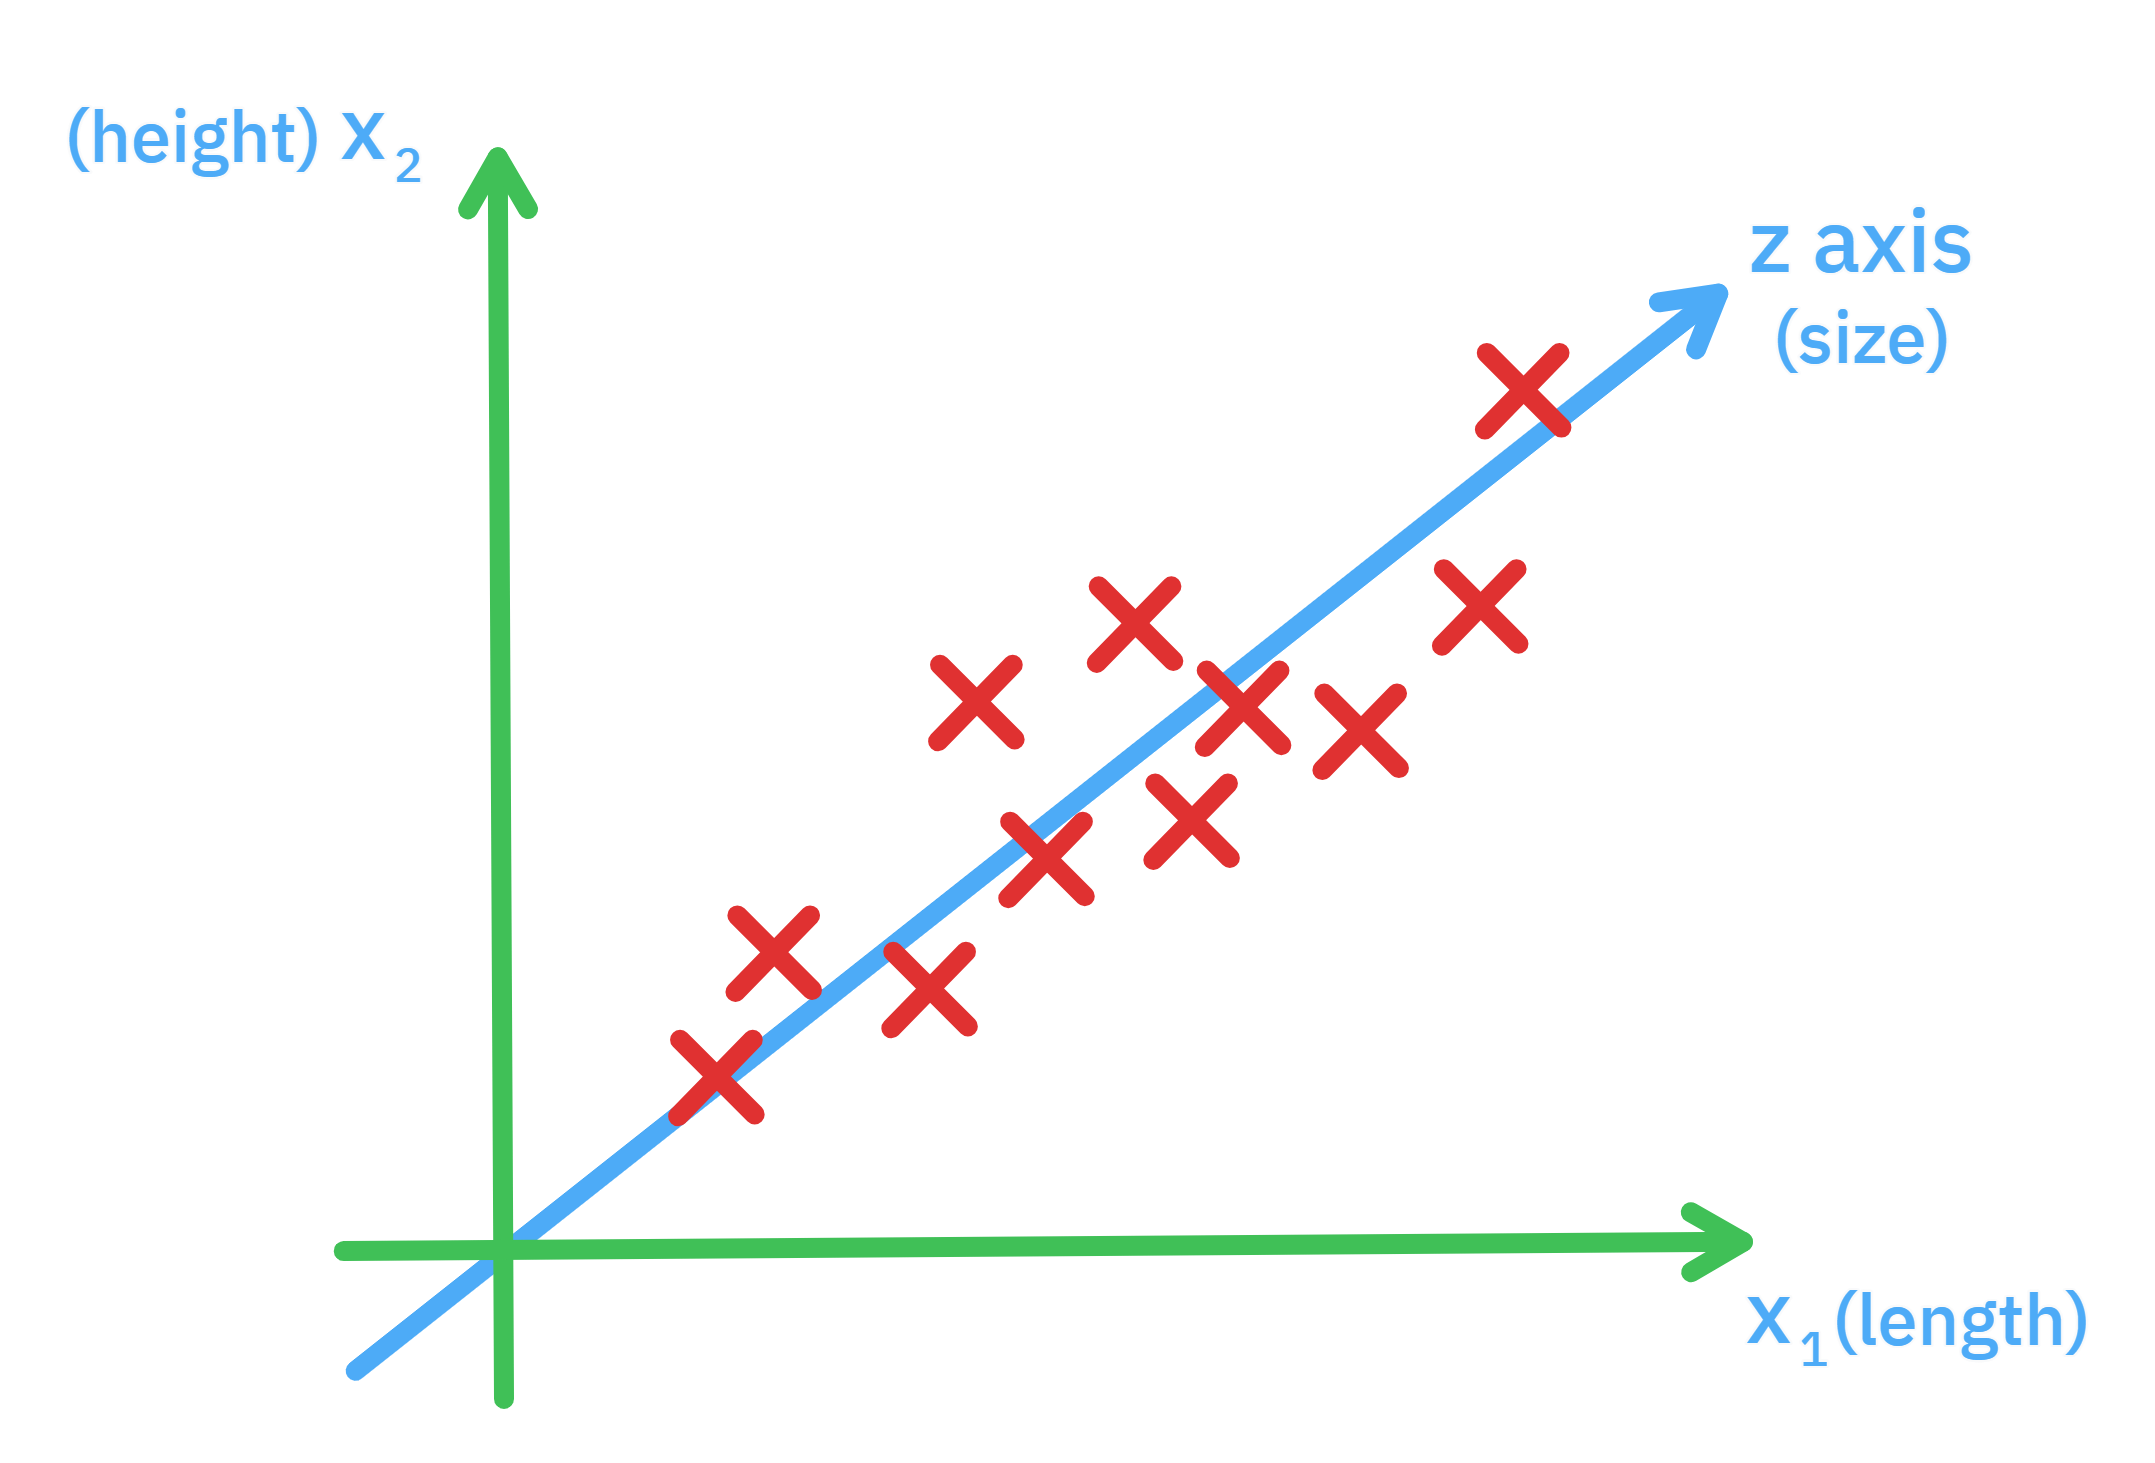
\includegraphics[width=0.7\textwidth]{graphics/pca.png}
\end{center}

\subsubsection{PCA in scikit-learn}

We can use scikit-learn to implement PCA in code. First, we perform feature scaling as an optional pre-processing. Then we can use \verb|fit| function to fit the data to obtain 2 or 3 new axes (principal components). There is an optional step in which we can examine how much variance is explained by each principal component using \verb|explained_variance_ratio|. In the final step, we use the \verb|transform| function to project the data onto the new axes. A code example is given here:

\begin{lstlisting}[language=Python]
X = np.array([[1, 1], [2, 1], [3, 2], [-1, -1], [-2, -1], [-3, -2]])
pca = PCA(n_components=1)
pca.fit(X)
pca.explained_variance_ratio_
X_trans = pca.transform(X)
X_reduced = pca.inverse_transform(X_trans)
\end{lstlisting}

\section{Week 3: Reinforcement Learning}

The idea of reinforcement learning is the same idea as training a dog: by a reward system. You reward the dog (called \textbf{agent}) when it behaves well (positive \textbf{action}) and you punish it when it does something wrong (negative action). In more technical words, Reinforcement Learning is a feedback-based Machine learning technique in which an agent learns to behave in an environment by performing the actions and seeing the results of actions. Reinforcement Learning has a lot of applications like controlling robots, factory optimization, financial (stock) trading, and playing games (including video games). 

\subsection{Return, Policy, and Markov Decision Process}

A reinforcement learning model consists of a number of \textbf{states}. An agent can only be in one state ($s$) at a time. Then it can take some \textbf{action} that bring it to another state ($s'$). Each state is associated with a number called \textbf{reward} denoted by $R(s)$. Some states are defined to be \textbf{terminal states} in which the agent will stop at the end. Suppose the agent starts from state $s_0$ and goes through states $s_1$, $S_2$, and so on (until a terminal state). Then the \textbf{return} is calculated as follows:
\[\textbf{Return} = R(s_0) + \gamma R(s_1) + \gamma^2 R(s_2) + \gamma^3 R(s_3) + \dots = \sum_{i=0}^{t} \gamma^i R(s_i)\]
where $t$ is the terminal state and $\gamma$ is the \textbf{discount factor} and is used to make the agent impatient (to make it prefer a sooner smaller reward to a later larger reward).

In order to make a decision in each state, we define \textbf{policy} which is a function $\pi(s) = a$ mapping from states to actions, that tells us what action $a$ to take in a given state $s$. The goal of a reinforcement learning model is to find a policy $\pi$ that tells you what action to take in every state so as to maximize the return.

\subsubsection{Markov's Decision Process (MDP)}

Markov’s Decision Process is a Reinforcement Learning policy used to map a current state to an action where the agent continuously interacts with the environment to produce new solutions and receive rewards. Markov’s Process states that the future is independent of the past, given the present. This means that, given the present state, the next state can be predicted easily, without the need for the previous state.
\begin{center}
    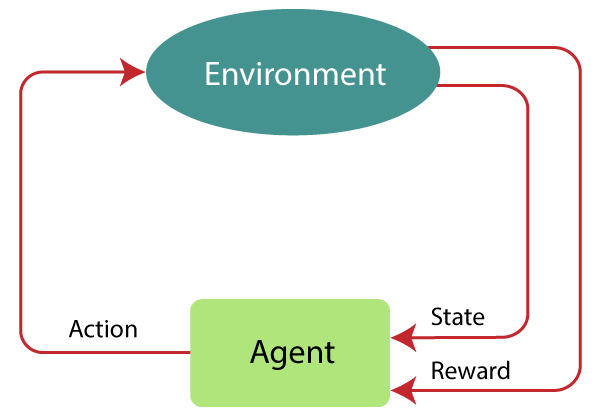
\includegraphics[width=0.55\textwidth]{graphics/MDP.png}
\end{center}

\subsection{State-Action Value Function (Q-Function)}

There's a key quantity that reinforcement learning algorithms try to compute which is called the state-action value function. We denote this function by $Q(s, a)$ and is defined as the \textbf{return if you start in state $s$, take action $a$ once, and then behave optimally} after that till you get to a terminal state. If you have a way to compute $Q(s, a)$ for every state, then all you need to do in a given state $s$ is to choose an action $a$ that maximizes the $Q(s, a)$. This means that given the Q-Function, our policy is defined as: \[\pi(s) = \text{arg}\max_a Q(s, a)\]

There is a key equation in reinforcement learning that helps us to compute the Q-function called \textbf{Bellman equation}. If $s$ and $a$ are current state and action, $s'$ is the state you get to after taking action $a$, and $a'$ is the action you take in state $s'$, then the Bellman equation expresses that: \[Q(s, a) = R(s) + \gamma \max_{a'} Q(s', a')\] In stochastic (random) environments, the goal is to maximize the expected return and the Bellman equation becomes \[Q(s, a) = R(s) + \gamma \, \mathbb{E}[\max_{a'} Q(s', a')]\]

\subsection{Deep Q-Learning for Continuous State Spaces}

In real-life situations, the states are in continuous spaces. For example, the state of a moving particle (like a helicopter) is defined as its position in space ($x, y, z$) and its instantaneous speed ($\Dot{x}, \Dot{y}, \Dot{z}$). The idea here to calculate $Q(s, a)$ is to use a neural network that gets $s$ and $a$ as an input vector $\Vec{x} = \binom{s}{a}$ and outputs $Q(s, a)$. This method is called \textbf{Deep Q-Network (DQN)}.

In order to train this neural network, we need training examples $(x^{(i)}, y^{(i)})$. We let the agent take action and get feedback each time, Thus in each trial, we get a tuple $(s^{(i)}, a^{(i)}, R(s^{(i)}), s'^{(i)})$ from which we can calculate $x^{(i)}$ and $y^{(i)}$ using Bellman equation:
\[x^{(i)} = \begin{bmatrix}
    s^{(i)} \\
    a^{(i)} \\
\end{bmatrix}, \qquad \qquad y^{(i)} = R(s^{(i)}) + \gamma \max_{a'} Q(s'^{(i)}, a')\]
You may wonder how is it possible to use the Q-Function during the training process. The answer is that at first, we don't know what is $Q(s, a)$. So we initialize the neural network randomly as a guess. The training process algorithm is given here:

\begin{algorithm}
\caption{Deep Q-Learning}
\begin{algorithmic} [1]
\State Initialize neural network randomly as guess of $Q(s, a)$
\Repeat
    \State Take action by agent and get $(s, a, R(s), s')$
    \State Store 10,000 most recent $(s, a, R(s), s')$ tuples
    \State Calculate $x^{(i)}$ and $y^{(i)}$ from $(s^{(i)}, a^{(i)}, R(s^{(i)}), s'^{(i)})$
    \State Train $Q_{new}$ such that $Q_{new} (s, a) \approx y$
    \State $Q \gets Q_{new}$
\Until{convergence}
\end{algorithmic}
\end{algorithm}

You may have noticed that in line 3 of the above algorithm, we have to take action while still learning. We can take actions randomly which turns out to be not a good idea. We can also pick the action $a$ that maximizes $Q(s, a)$. There is another way to choose actions that turns out to be very effective called \textbf{$\mathbf{\epsilon}$-greedy policy}. In this method, we have two concepts \textbf{Exploitation} and \textbf{Exploration}. In each state, we choose one of the following ways:
\begin{itemize}
    \item \textbf{Exploitation:} With probability of $1-\epsilon$, pick the action $a$ that maximizes $Q(s, a)$
    \item \textbf{Exploration:} With probability of $\epsilon$, pick an action $a$ randomly
\end{itemize}
This random action picking helps to solve the problems occurring in the random initialization of the neural network. Since the Q-Function gets better and better during the training process, it is common to start with a high $\epsilon$ and then gradually decrease it. This makes our model choose more random actions at first when the Q-function is not as accurate.

\subsubsection{Improved Neural Network Architecture}

You may have noticed that in order to find $\max_{a} Q(s, a)$ we have to run the inference $n$ times ($n$ is the number of actions) for each action and then find the maximum case. In order to fix that problem, we can change the architecture of our network to get only $s$ as input and output $n$ numbers as $Q(s, a_1), Q(s, a_2), \dots, Q(s, a_n)$. This improvement will result in much more efficient inference. 

\subsubsection{Limitations of Reinforcement Learning}

Reinforcement learning has an exciting research direction with potential for future application, but at the moment it has some limitations. For instance, it is much easier to get it to work in a simulation environment than a real robot and it also has fewer applications than supervised and unsupervised learning.

\end{document}
